\documentclass[12pt,a4paper, twoside]{report}

% Import preamble and setup code
% Packages and setup code
\usepackage{graphicx}
\usepackage{caption}
\usepackage{fancyhdr}
\usepackage{geometry}
\usepackage{lipsum}
\usepackage{xcolor}
\usepackage{pagecolor}
\usepackage{chemformula}
\usepackage{url}
\usepackage{orcidlink}
\usepackage{cleveref}
\usepackage{tabularx}
\usepackage{makecell}
\usepackage{array}
\usepackage{float}      % For the [H] specifier to force the table to stay in place
\usepackage{booktabs}   % For \toprule, \midrule, \bottomrule
\usepackage{multirow}   % For \multirow\usepackage{longtable}
\usepackage{appendix}
\usepackage{helvet} % Use Helvetica font
\usepackage[backend=biber,style=numeric,sorting=none]{biblatex}
\addbibresource{bibliography.bib} 

\usepackage{hyperref}
\hypersetup{
  colorlinks=true,
  allcolors=black,
  pdfborder={0 0 0},
  }
  
  % Page geometry
  \geometry{
    a4paper,
    left=3.2cm,
    right=3.2cm,
    top=3.2cm,
    bottom=3.2cm,
    headheight=14pt
    }
    
    \usepackage{fancyhdr}
    \pagestyle{fancy}
    \fancyhf{} % Clear existing header/footer settings
    \fancyhead[LE,RO]{\small\leftmark} % Chapter title on even and odd pages in small caps
    \fancyfoot[C]{\thepage} % Centered page number at the bottom of each page
    
    
% Indentation    
\setlength\parindent{0pt} % Set no indentation for the entire file
\newcommand{\myindent}{\hspace*{2em}}


% Define how chapter titles appear in headers in all caps
\renewcommand{\chaptermark}[1]{\markboth{\scriptsize\MakeUppercase{Chapter \thechapter.\ #1}}{}}


% Define the custom \todo{} command
\newcommand{\todo}[1]{\textcolor{red}{TODO: #1}}



% Define variables for Author Name and Thesis Title
\newcommand{\AuthorName}{Christine Annelise Midtgaard} 
\newcommand{\ThesisTitle}{Exploring Deep Learning Techniques for Long-Tailed Recognition: Methods, Models, and Analysis}

\newcommand{\SupervisorName}{Kim Bjerge}

% Custom patch to suppress page number on \part pages
\makeatletter
\let\sv@endpart\@endpart
\def\@endpart{\thispagestyle{empty}\sv@endpart}
\makeatother




% Begin document
\begin{document}
\emergencystretch 3em
% Roman numeral page numbering for front matter
\pagenumbering{roman}

% Title page
\begin{titlepage}
    \centering
    \vspace*{-0.8cm}
    
    % Line above title
    \rule{\linewidth}{0.3mm} % Adjust thickness as needed
    \vspace{1pt}
    % Thesis Title
    {\LARGE\bfseries \ThesisTitle \par}
    \vspace{0.3cm}

    % Thesis Type and Field
    {\small\textsc{Master’s Thesis in\\
    Electrical Engineering}\par}

    \vspace{1pt}
    % Line below title
    \rule{\linewidth}{0.3mm} % Adjust thickness as needed
    \vspace{0.2cm}
    
    % Author information
    {\small \textsc{By}\\[0.4cm]
    \normalsize \textbf{\AuthorName}\\
    \small \textsc{au521655\\
    Study Program: Electrical Engineering}\par} %Change name in preamble.tex
    \vspace{1cm}
    
    % Supervisor Information
    {\small \textsc{Supervisor}\\
    \normalsize \textbf{\SupervisorName}\\
    \small \textsc{Associate Professor}\\
    kbe@ece.au.dk\par}
    \vspace{1.5cm}

    
    % University Logo
    
\includegraphics[width=0.38\textwidth]{Logo/aulogoblue.png}\par
    \vspace{1.2cm}

    
    % University and Department Information
    {\textsc{M.Sc. in Electrical Engineering\\
    Department of Engineering
    Science \& Technology\\
    Aarhus University}}\par
    \vspace{.8cm}
    
    % Defense Date
    {\normalsize \textsc{January 3, 2025}}
\end{titlepage}


\newpage
\thispagestyle{empty} % Removes header/footer from the blank page
\mbox{} % Inserts an empty box to force the page
\newpage

% Abstract, Acknowledgment
\chapter*{Abstract}
\addcontentsline{toc}{chapter}{Abstract}
Long-tailed datasets, where a few classes dominate with abundant samples while many classes have sparse representation, pose significant challenges for traditional training methods. These imbalances often lead to models that perform well on majority classes but struggle to recognize or generalize to minority (tail) classes.

% This thesis focuses on evaluating and implementing re-weighting methods for long-tailed learning, as outlined in the survey Deep Long-Tailed Learning: A Survey by Zhang et al. The methodologies explored include advanced sampling strategies, re-weighted loss functions, and modifications to deep learning architectures tailored to imbalanced data.

% A unique application of these methods is demonstrated on a custom dataset of moth images collected near the equator, where the goal is accurate species identification. Through a series of experiments, the thesis investigates how different approaches to long-tailed learning impact model performance across head, middle, and tail classes.

% The findings contribute to understanding the efficacy of these methods and provide insights into best practices for handling real-world long-tailed datasets.


\chapter*{Acknowledgements}
\addcontentsline{toc}{chapter}{Acknowledgements}
I would like to thank my supervisor, \SupervisorName, for their guidance, constructive feedback, and inspiring conversations throughout the development of this thesis. I am also deeply thankful to my family for providing me with room for my frustrations, and for cooking meals during the challenging times of this journey. I want to thank my friend, Line, for her valuable insights in writing a thesis. A special thanks to boyfriend for his outstanding patience and understanding.

% Table of Contents
\tableofcontents
\newpage
\printglossary[type=\acronymtype, title=List of Acronyms]

\newpage
% Switch to Arabic numerals starting from Chapter 1
\newpage
\pagenumbering{arabic}

% Chapters
\chapter{Introduction}
%\section{Introduction}
\lipsum[3-5] \cite{mbakidi2022a}
\section{Methodology}
\lipsum[3-5]
\section{Results}
\lipsum[3-5]
\section{Discussion}
\lipsum[3-5]
\section{Conclusion}
\lipsum[3-5]


\chapter{Background}
% Chapter 2: Background

% Length: aim for 10-15 pages

This chapter presents the different background topics of the thesis work, which are the long-tailed datasets, model architectures \textit{Convolutional Neural Networks (CNN)} and \textit{Visual Transformers (VT)}, the deep long-tailed learning methods \textit{Class Re-balancing (CR)}, \textit{Information Augmentation (IA)}, 
and \textit{Module Improvement (MI)}. These topics will be explained for the reader.\\

Mention image classification, as it is the primary goal of this thesis. 

\section{Long-Tailed Datasets}
Long-tailed datasets pose significant challenges in deep learning, as they represent an extreme form of class imbalance. Addressing these challenges is central to this thesis, which explores methods to improve model performance on underrepresented classes. This section outlines the structure of long-tailed distributions and their implications.

A balanced dataset is one where all classes are evenly represented, whereas imbalanced datasets feature varying sample sizes across classes. Long-tailed datasets are characterized by a significant class imbalance, where a few dominant classes account for most samples (head classes), while the majority of classes are underrepresented (tail classes) as depicted in Figure \ref{fig:lt_distribution}. This  distribution is common for real-world datasets \cite{Newman_2005, liu2019largescalelongtailedrecognitionopen}. For example, the iNaturalist, a popular benchmark for image classification, exhibits a long-tailed distribution of species \cite{vanhorn2018inaturalistspeciesclassificationdetection}. Other benchmarks are constructed by sampling from datasets such as ImageNet \cite{ImageNet2009} and CIFAR-100 \cite{krizhevsky2009learning} using a Pareto distribution, which simulates long-tailed class distributions with a power-law decay \cite{zhang2023deep, dealvis2024surveydeeplongtailclassification,cao2019learningimbalanceddatasetslabeldistributionaware}.

One such benchmark, CIFAR100-LT \cite{cao2019learningimbalanceddatasetslabeldistributionaware}, derived from the CIFAR-100 dataset \cite{krizhevsky2009learning}, serves as the primary dataset for the experiments conducted in this thesis. CIFAR-100 is a widely used benchmark in classification research due to its diverse class representation and manageable size. It consists of 60,000 32x32 color images divided into 100 classes, each with 600 samples. These are further split into 500 training images and 100 testing images per class. CIFAR100-LT is created by reducing the number of samples in certain classes of CIFAR-100 following a Pareto distribution, introducing significant class imbalance. This makes it an ideal benchmark for studying the challenges posed by long-tailed datasets.  

\begin{figure}[ht]
    \centering
    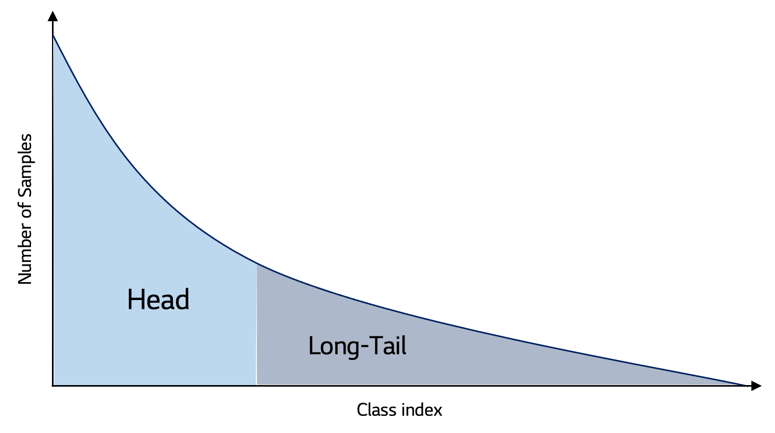
\includegraphics[width=0.8\textwidth]{Images/long_tail_distribution.png} 
    \caption{Illustration of a long-tailed distribution. Figure from \cite{lgresearch257}.}
    \label{fig:lt_distribution} % Use a unique label for referencing the figure
\end{figure}

Class imbalance has a profound impact on model performance compared to evenly distributed datasets \cite{vanhorn2017deviltailsfinegrainedclassification, cui2019classbalancedlossbasedeffective}. Deep networks trained on long-tailed datasets often exhibit biased performance, favoring head classes while performing poorly on tail classes \cite{zhang2023deep}. Zhang et al. (2023) provide a comprehensive survey of methods addressing this challenge, categorizing current approaches into three main groups: class re-balancing, information augmentation, and module improvement. These methods will be further explored in section \ref{sec:lt_methods}. 

\section{Model Architechtures}
Describe the role of deep learning models in handling long-tailed datasets.

\subsection{Convolutional Neural Networks}
Add historical context.
Mention specific CNNs used in this thesis (e.g., ResNet, MobileNet).

\subsection{Visual Transformers}
Explain their advantages over CNNs for certain tasks.
Mention why they are relevant for handling long-tailed datasets.


\section{Classic Long-Tailed Methods}
\label{sec:lt_methods}
Introduce the three methods (CR, IA, MI) with a brief explanation of their purpose.\\

Following the paper \textit{Deep Long-Tailed Learning: A Survey} \cite{zhang2023deep}, the existing deep long-tailed learning methods are grouped into three main categories based on their technical approach: class re-balancing, information augmentation, and module improvement. These categories are further divided onto sub-categories: re-sampling, class-sensitive learning, logit adjustment, transfer learning, data augmentation, representation learning, classifier desing, decoupled training, and ensemble learning as shown on figure \ref{fig:lt_main_categories}. This thesis does not aim to examine all the beforementioned method, but aims to find a deep learning approach to a specific problem. The backgrounds of the methods used in this thesis are described in this section.

\begin{figure}[ht]
    \centering
    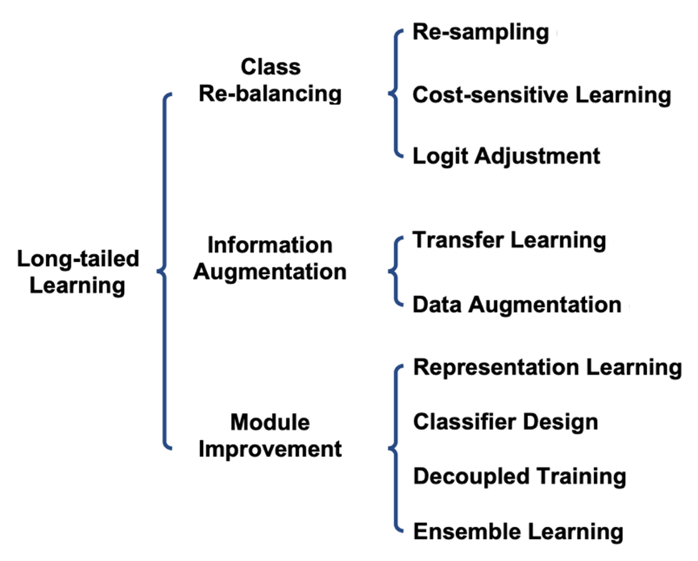
\includegraphics[width=0.8\textwidth]{Images/lt_methods_categories.png} 
    \caption{Long-tailed categories as described by \textit{Zhang et al.} \cite{zhang2023deep}.}
    \label{fig:lt_main_categories} % Use a unique label for referencing the figure
\end{figure}

\subsection{Class Re-balancing}
The class re-balancing method aims to re-balance the effect of the imbalanced training dataset, and has three main sub-categories: re-sampling, class-sensitive learning, and logit adjustment \cite{zhang2023deep}. 

\subsubsection{Re-sampling}
The traditional way to sample when training deep networks is bases on mini-batch gradient descent with random sampling. This means that each sample has an equal probability of being sampled. When sampling from an imbalanced dataset, samples from head classes naturally occur more often, and thus have higher chance of being sampled than samples from tail classes, making the resulting deep models biased towards head classes. Re-sampling is a method that adresses this problem by adjusting the number of samples per class in each sample batch for model training. 

\subsubsection{Class-sensitive Learning}
Class-sensitive learning incorporates strategies to adjust the loss function, making it more sensitive to the imbalanced nature of the dataset. This approach directly modifies the optimization process to prioritize learning from under-represented tail classes.

TODO: Mention re-weighting and re-margining.
Table/overview of loss functions as in the paper.


\subsubsection{Loss Functions for Class-Sensitive Learning}
The loss function serves as a measure of the model's fitness to the data, quantifying the distance between the actual and predicted values of the target. Typically, the loss is represented as a nonnegative value, where smaller values indicate a better fit, and a perfect fit corresponds to a loss of zero \cite{zhang2023dive}.

Conventional training of deep networks using the softmax cross-entropy loss often overlooks class imbalance. This results in uneven gradients for different classes, leading to suboptimal performance on underrepresented classes. To mitigate this issue, modifications to the loss function are introduced to ensure a more balanced contribution from each class during training. One such technique is re-weighting which adjusts the training loss for different classes by assigning a specific weight to each class \cite{zhang2023deep}. The softmax cross-entropy loss is used as a baseline, and is described below along with the loss functions for re-weighting.

\myindent \textbf{Softmax Cross-Entropy Loss}
The \textit{Softmax-Cross-Entropy loss}, often referred to as \textit{softmax loss}, is a widely used combination for training deep neural networks in classification tasks, including image classification. It is particularly effective for multi-class problems, where the goal is to assign an input image to one of several predefined categories \cite{cs231n} \cite{pytorch_crossentropy}.

The \textit{Softmax} function transforms the raw output scores (logits) of the final layer of a neural network into a probability distribution over \( K \) classes. For an input \( \mathbf{z} = [z_1, z_2, \dots, z_K] \), the Softmax function for class \( i \) is defined as:

\begin{equation}
    P(y = i \mid \mathbf{z}) = \frac{\exp(z_i)}{\sum_{j=1}^{K} \exp(z_j)}
\end{equation}

Here, \( \exp(z_i) \) ensures that all values are positive, and dividing by the sum normalizes the probabilities so that they sum to 1. This normalization is crucial for classification, as it allows the network's outputs to represent the likelihood of each class.

The \textit{Cross-Entropy loss} measures the difference between the predicted probability distribution \( \mathbf{P} \) (produced by Softmax) and the true distribution \( \mathbf{y} \) (the one-hot encoded ground truth). It is defined as:

\begin{equation}
    \mathcal{L}_{\text{CE}} = -\sum_{i=1}^{K} y_i \log(P(y = i \mid \mathbf{z}))
\end{equation}


For a single example where the true class is \( c \), this simplifies to:

\begin{equation}
    \mathcal{L}_{\text{CE}} = -\log(P(y = c \mid \mathbf{z}))
\end{equation}


This formulation penalizes incorrect predictions by heavily weighting the log of the predicted probability for the true class. The loss is minimized when the predicted probability \( P(y = c \mid \mathbf{z}) \) approaches 1, indicating high confidence in the correct class.

This combination has become the de facto standard for image classification tasks, providing a robust and mathematically sound framework for training deep neural networks.


\myindent \textbf{Weighted Softmax Cross-Entropy Loss}
The \textit{Weighted Softmax Cross-Entropy loss}, often referred to as \textit{weighted softmax loss}, is a variant of the standard softmax cross-entropy loss, designed to address imbalanced datasets \cite{pytorch_crossentropy} \cite{lin2018focallossdenseobject}. By assigning different weights to each class, this method ensures that underrepresented classes contribute more to the overall loss, improving the model's performance on minority classes. The weighted cross-entropy loss applies class-specific weights to the standard cross-entropy formulation. It is defined as:

\begin{equation}
    \mathcal{L}_{\text{WCE}} = -\sum_{i=1}^{K} w_i y_i \log(P(y = i \mid \mathbf{z}))
\end{equation}

Where \( w_i \) is the weight for class \( i \), reflecting its relative importance, \( y_i \) is the one-hot encoded true label for class \( i \), and \( P(y = i \mid \mathbf{z}) \) is the predicted probability for class \( i \).

For a single example where the true class is \( c \), the loss simplifies to:

\begin{equation}
    \mathcal{L}_{\text{WCE}} = -w_c \log(P(y = c \mid \mathbf{z}))
\end{equation}

This weighted formulation ensures that minority classes contribute more to the overall loss, addressing the imbalance during training and improving the model's performance on underrepresented classes.

\myindent \textbf{Focal Loss}
Focal Loss, introduced by Lin et al. (2017) \cite{lin2018focallossdenseobject}, addresses the challenges of extreme class imbalance in classification tasks by dynamically scaling the standard cross-entropy loss. Focal Loss mitigates the issue of imbalanced datasets by down-weighting the loss contributions from well-classified examples and focusing on misclassified examples during training.

% For multiclass classification, the focal loss is formulated as:

% \begin{equation}
%     \mathcal{L}_{\text{FL}} = - \frac{1}{N} \sum_{i=1}^{N} \sum_{c=1}^{K} \alpha_c (1 - p_{i,c})^\gamma \log(p_{i,c}),
% \end{equation}

% where \( N \) is the number of samples, \( K \) is the total number of classes, \( p_{i,c} \) is the predicted probability for class \( c \) for the \( i \)-th sample, typically obtained via a softmax function, \( \alpha_c \) is a weighting factor for class \( c \), \( \gamma \geq 0 \) is the focusing parameter, which adjusts the scaling effect of \( (1 - p_{i,c})^\gamma \). A higher \( \gamma \) increases the model's focus on harder examples, and \( \log(p_{i,c}) \) is the standard cross-entropy loss for the true class.


% The term \( (1 - p_{i,c})^\gamma \) serves as a modulating factor that reduces the contribution of well-classified examples, where \( p_{i,c} \) is high, to the total loss. This enables the model to focus more on examples with lower predicted probabilities, which are typically harder to classify. The parameter \( \alpha_c \) further adjusts the loss to account for class imbalance, ensuring that minority classes receive adequate attention during training.


\myindent \textbf{Class-Balanced Loss} \textit{Class-balanced loss}, introduced by Cui et al. (2019) \cite{cui2019classbalancedlossbasedeffective}, ...

\myindent \textbf{Balanced Softmax Loss} \textit{Balanced Softmax loss}, introduced by Ren et al. (2020) \cite{ren2020balancedmetasoftmaxlongtailedvisual}, ...

\myindent \textbf{LDAM Loss} \textit{LDAM loss}, introduced by Cao et al. (2019) \cite{cao2019learningimbalanceddatasetslabeldistributionaware}, ...

\myindent \textbf{Equalization Loss} \textit{Equalization loss}, introduced by Tan et al. (2020) \cite{tan2020equalizationlosslongtailedobject}, ...


\subsection{Information Augmentation}
Data augmentation techniques tailored for long-tailed datasets.

\subsubsection{Transfer Learning}

\subsubsection{Data Augmentation}



\subsection{Module Improvement}
Architectural changes to improve tail-class representation.

\chapter{Methodology}
% Chapter 3: Methodology

This chapter describes the methods and approaches used in the experiments. This includes the selection of dataset, models, loss functions, as well as training and evaluation strategies.

\section{Overview of Approach}

Image classification involves predicting the correct category of an image from a set of predefined classes. This project focuses on addressing the challenge of class imbalance, where some classes have many samples while others have very few.

The CIFAR-100 dataset \cite{krizhevsky2009learning} was chosen because it is small enough to work with efficiently and is commonly used in other research. To create a long-tailed version of the dataset, its class distribution was adjusted to match the distribution of the ImageNet-LT dataset used in \cite{zhang2023deep}. This adjustment ensures that the experiments simulate real-world class imbalance.

Several loss functions designed to handle class imbalance were tested in this project, including Softmax Cross-Entropy (CE), Focal Loss (FL), Class-Balanced (CB) Loss, Balanced Softmax (BS) Loss, Equalization (EQ) Loss, and LDAM Loss. These loss functions modify how the models learn, making it easier for them to focus on classes with fewer samples.

The experiments were performed using four model architectures: ResNet50, MobileNetV2, ConvNeXt Base, and ViT-B/16. All models were pretrained on ImageNet, which provided a strong starting point for fine-tuning on the CIFAR-100 dataset. These models were chosen because they are well-suited for image classification tasks and represent different design approaches.

Each model was trained on both a balanced training set and a long-tailed training set. The performance of the models was evaluated using a balanced test set, a long-tailed test set, and the long-tailed test set divided into head, middle, and tail classes. This division made it possible to analyze the performance for classes with different numbers of samples. The main evaluation metric used was top-1 accuracy, which measures how often the model's top prediction is correct.

In what follows, each step of the methodology will be explained in detail.

\section{Dataset Preparation and Specifications}
\label{sec:dataset_specs}
Following the dataset structure used in \textit{Deep Long-Tailed Learning: A Survey}, the CIFAR100 dataset was modified to create a long-tailed training set and a balanced test set. 

\subsection{Benchmark Dataset Selection}
There are a number of benchmark datasets for long-tailed image classification tasks, including ImageNet-LT \cite{liu2019largescalelongtailedrecognitionopen}, Places365-LT \cite{liu2019largescalelongtailedrecognitionopen}, CIFAR-100-LT \cite{cao2019learningimbalanceddatasetslabeldistributionaware}, and iNaturalist 2018 \cite{vanhorn2018inaturalistspeciesclassificationdetection}. The previous three are sampled from ImageNet, Places365, and CIFAR-100, following the Pareto distribution, as described in section \ref{sec:lt-datasets}, while the iNaturalist 2018 is a natural long-tailed dataset. Table \ref{tab:datasets} summarizes the four datasets and their data specifications. 

\begin{table}[ht]
    \centering
    \caption{Summary of long-tailed benchmarks for image classification.}
    \begin{tabular}{lccc}
    \hline
    \textbf{Dataset}           & \textbf{\# Classes} & \textbf{\# Training Data} & \textbf{\# Test Data} \\ \hline
    ImageNet-LT \cite{liu2019largescalelongtailedrecognitionopen}  & 1,000              & 115,846                   & 50,000                \\
    CIFAR-100-LT \cite{cao2019learningimbalanceddatasetslabeldistributionaware}  & 100                & 50,000                    & 10,000                \\
    Places-LT  \cite{liu2019largescalelongtailedrecognitionopen}   & 365                & 62,500                    & 36,500                \\
    iNaturalist 2018 \cite{vanhorn2018inaturalistspeciesclassificationdetection} & 8,142            & 437,513                   & 24,426                \\ \hline
    \end{tabular}
    \label{tab:datasets}
\end{table}
    

With its 100 classes and only 60,000 samples, the CIFAR-100 dataset was chosen as a benchmark for the experiments conducted in this thesis based on its managable size, compared to the other benchmarks, and widespread use as a standard in image classification research. Its comparatively small size allows for rapid experimentation and comparisons, wheras a larger benchmark requires more computational effort and time for experiments, thus it is well-suited for multiple configurations and evaluations. However, CIFAR-100 has some limitations compared to larger dataset, like ImageNet-LT or iNaturalist. For example, CIFAR-100 images are of relatively low resolution ($32 \times 32$ pixels), as depicted in Figure \ref{fig:cifar100_images}, compared to ImageNet ($224 \times 224$ pixels), and may limit the ability of models to capture fine-grained details. Likewise, the smaller number of classes and samples can result in less diversity compared to datasets like iNaturalist 2018, which contains nearly nine times as many samples in the training data as CIFAR-100-LT. Despite these drawbacks, CIFAR-100-LT remains a practical choice for this thesis due to its computational efficiency. 

\begin{figure}[h!]
    \centering
    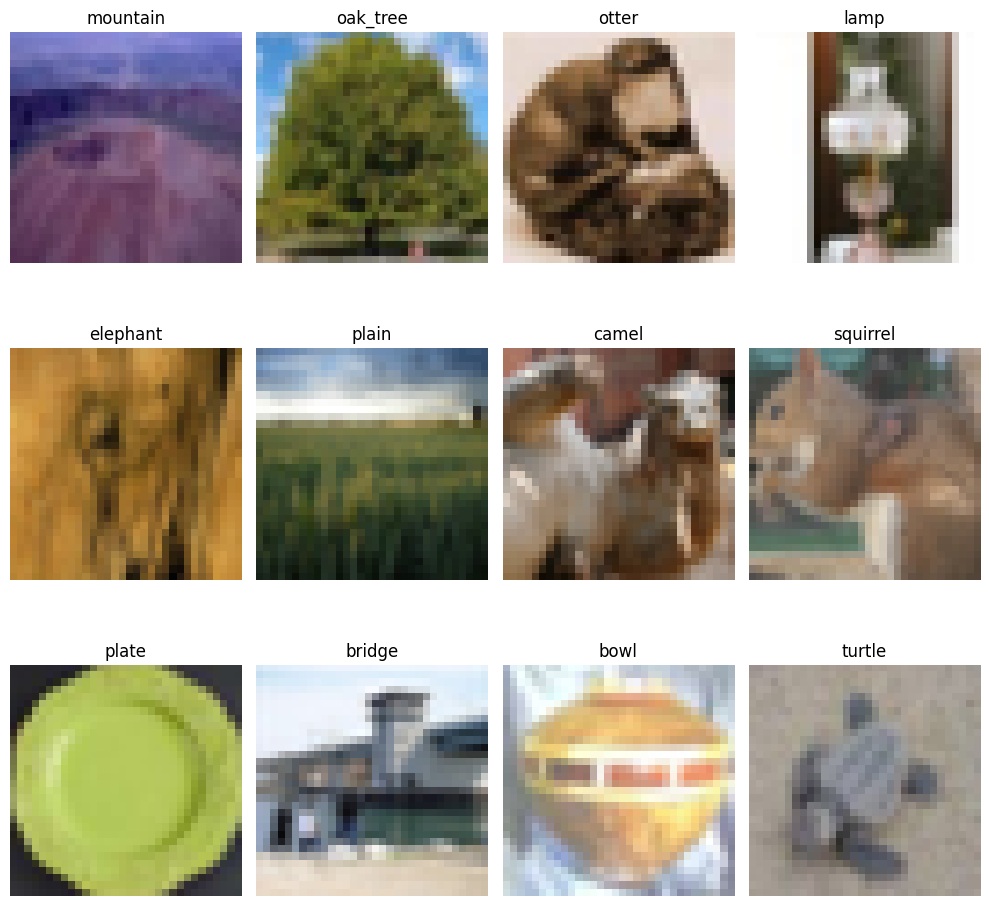
\includegraphics[width=0.5\textwidth]{Images/cifar100_sample_grid.png}
    \caption{Examples from the CIFAR-100 dataset showing the low resolution ($32 \times 32$ pixels). Each image is labeled with its corresponding class name.}
    \label{fig:cifar100_images}
\end{figure}

\subsection{Data Characteristics: Class Distribution}
Understanding the class distribution in long-tailed datasets is essential for evaluating the impact of the class imbalance on model performance. This section analyzes the class distribution of the benchmark ImageNet-LT used in \cite{zhang2023deep}, which serves as a reference for creating a similar distribution across the CIFAR-100-LT training, evaluation, and test datasets.  

The ImageNet-LT dataset, introduced by Liu et al. \cite{liu2019largescalelongtailedrecognitionopen}, has been widely used in empirical studies, including \textit{Deep Long-Tailed Learning: A Survey} \cite{zhang2023deep}. The class distributions of its training set is plotted in figure \ref{fig:IN-train}. The ImageNet-LT is constructed from the original ImageNet-2012 following the Pareto-distribution (Eq. \eqref{eq:pareto}) with power value $\alpha=6$ \cite{liu2019largescalelongtailedrecognitionopen}, resulting in an imbalance ratio of 256, meaning that the most frequent class has 256 times more samples than the least frequent class. As suggested in figure \ref{fig:IN-train}, the most frequent class has 1280 images, and the least frequent class 5 images \cite{liu2019largescalelongtailedrecognitionopen}. The power value of 6 is relatively large, resulting in the steep imbalance and very few samples in the tail, as seen in figure \ref{fig:IN-train}. The underrepresentation in the tail classes poses a significant challenge for models to learn from tail classes. Both the validation and test sets are balanced with 20 samples per class in the validation set, and 50 samples per class in the test set. 


\begin{figure}[h!]
    \centering
    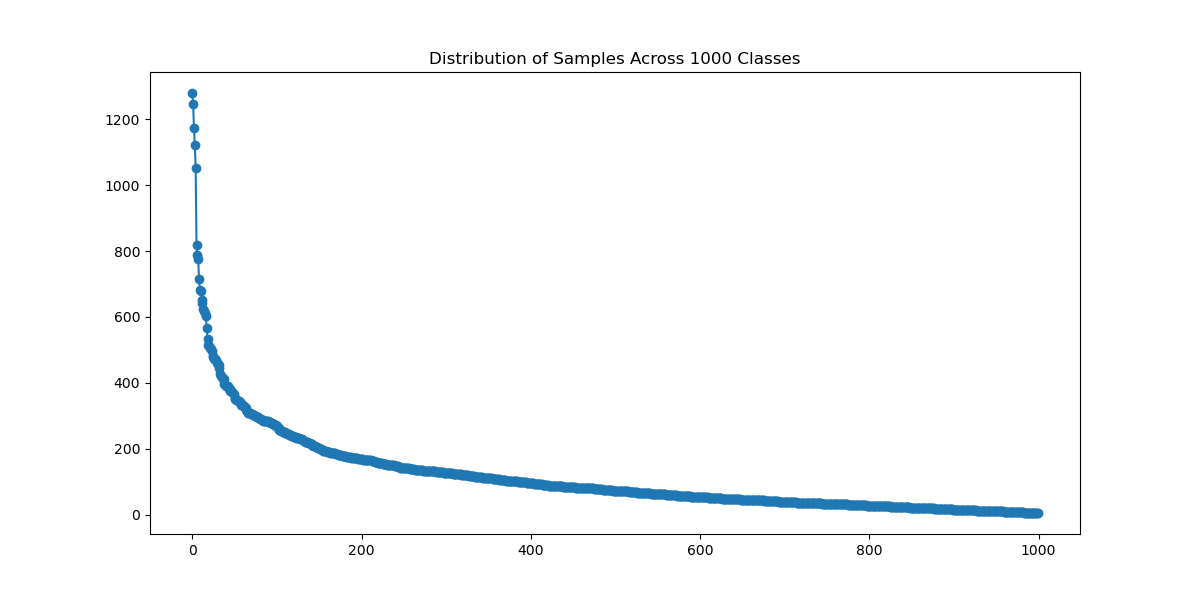
\includegraphics[width=0.9\textwidth]{Images/Plots/class_distribution_train.png}
    \caption{The class distribution of the training images for the ImageNet-LT dataset shows a long-tailed distribution.}
    \label{fig:IN-train}
\end{figure}


However, investigating the CIFAR-100-LT dataset used by Cao et al. \cite{cao2019learningimbalanceddatasetslabeldistributionaware} shows that the training dataset follows a exponential decay, and not a pareto distribution. The imbalance factor in their studies is 100, meaning that the most frequent class has 100 times more samples than the least frequent class, following equation \eqref{eq:exp}. This means that the imbalance is not as steep as with the Pareto distribution, resulting in a middle section of classes with fewer samples than the head classes, but more samples than the tail classes, see figure \ref{fig:cifar100_train_450_imb}. The following section will describe the preparation of CIFAR-100 for the experiments in this thesis.


\subsection{CIFAR-100-LT}
The experiments conducted in this thesis are trained and evaluated on the CIFAR-100 dataset. This was downloaded using with PyTorch \cite{pytorch_cifar100}. The training and test datasets were preprocessed by converting the images to tensors using the ToTensor transformation and saved as .pth files for efficient loading during experiments. 

The class distributions used in experiments in this thesis: Balanced training set, balanced test set, balanced validation set, long-tailed training set, long-tailed test set, long-tailed test set split into head, middle and tail. The class distributions can be seen in table \ref{tab:class_distributions}.

\begin{table}[h!]
    \centering
    \caption{Class Distributions Used in Experiments}
    \label{tab:class_distributions}
    \small
    \begin{tabular}{ll}
    \toprule
    \textbf{Dataset Type}                       & \textbf{\# Samples}                                                                 \\ \midrule
    Balanced Training Set                       & 45,000        \\ 
    Balanced Validation Set                     & 10,000    \\ 
    Balanced Test Set                           & 5,000    \\ \hline
    Long-Tailed Training Set                    & 9,754      \\ 
    Long-Tailed Test Set                        & 1,051 \\ \hline
    Head  & 844 \\ 
    Middle   & 169 \\ 
    Tail  & 38 \\
    \bottomrule
    \end{tabular}
    \end{table}
    

To address the needs of the experiments in this thesis, the original CIFAR-100 dataset was modified to create a new split from the training data. Specifically, the training data was split into 450 samples per class for training and 50 samples per class for testing, mirroring the test data for the ImageNet. The original test set of the CIFAR-100 dataset was retained as the validation set for evaluation during training. All datasets were saved locally to maintain reproducibility.

\textbf{Long-tailed Training Set:} To simulate real-world scenarios with class imbalances, the training dataset was modified to introduce an exponential imbalance across the 100 classes. Following the procedure of \cite{cao2019learningimbalanceddatasetslabeldistributionaware}, the imbalance was created using exponential decay. Here, the number of samples per class decreases exponentially, controlled by the imbalance factor, following equation \eqref{eq:exp}. For this thesis, an imbalance factor of 100 was applied. This means that the most frequent class contains a 100 times more samples than the least frequent class. 

\begin{figure}[h!]
    \centering
    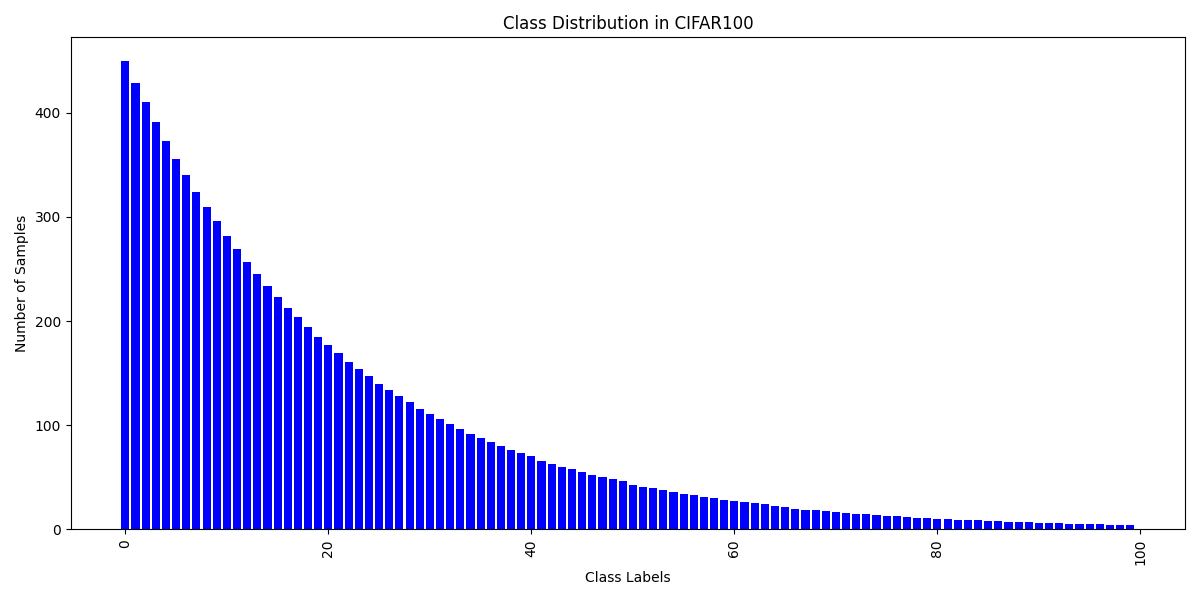
\includegraphics[width=0.9\textwidth]{Images/Plots/cifar100_train_450_imb.png}
    \caption{The class distribution of the CIFAR-100 long-tailed training set with 450 samples in the most frequent class.}
    \label{fig:cifar100_train_450_imb}
\end{figure}

The resulting class distribution varied from the most frequent class having 450 samples to the least frequent class having only 4 samples, as shown in figure \ref{fig:cifar100_train_450_imb}. This imbalance ensured no class was left with zero samples, maintaining the integrity of all classes for training. The dataset was saved locally to maintain reproducibility.


\textbf{Long-Tailed Test Set:} To evaluate the performance of the model under similar conditions to the imbalanced training set, an imbalanced test set was created from the previously split test dataset. The imbalance in the test set mirrors the exponential distribution used for the training data, with the same imbalance factor of 0.01. The class distribution in the test set follows the same order of classes (from most to least frequent) as the imbalanced training set. No class has fewer than one sample. The class distribution can be seen in figure \ref{fig:cifar100_test_imb}. The dataset was saved locally to maintain reproducibility.

\begin{figure}[h!]
    \centering
    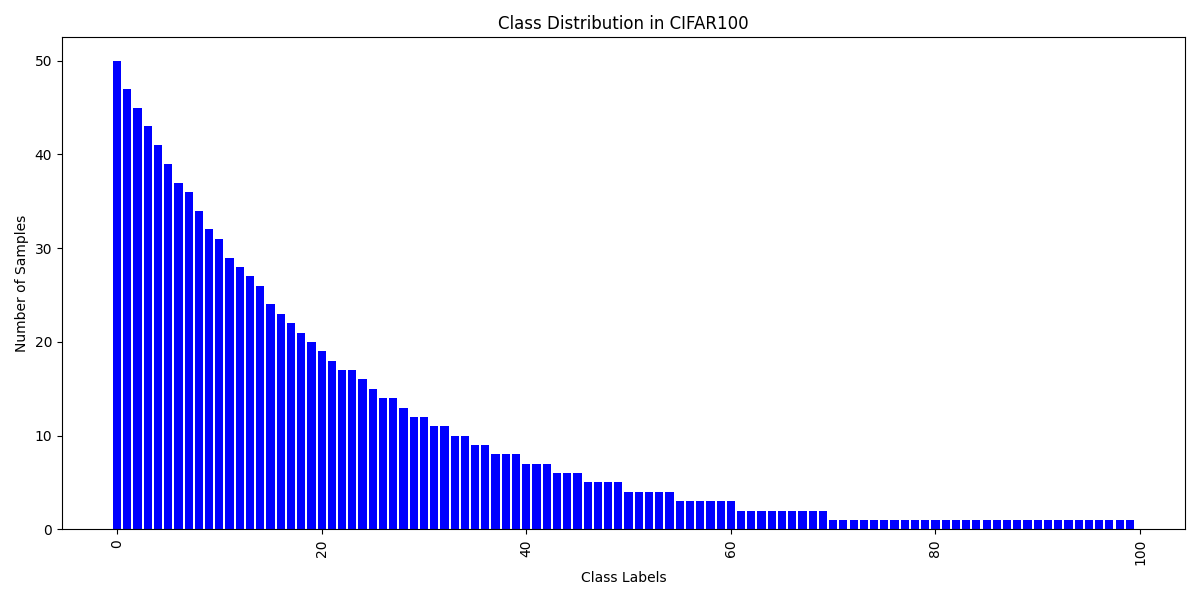
\includegraphics[width=0.9\textwidth]{Images/Plots/cifar100_test_imb.png}
    \caption{The class distribution of the CIFAR-100 long-tailed test set with 50 samples in the most frequent class.}
    \label{fig:cifar100_test_imb}
\end{figure}

To further analyze performance, the test set was divided into three subsets: head, middle, and tail classes, comprising of $1/3$ each (see table \ref{tab:class_distributions}). This categorization allows for a detailed evaluation of the methods across different classes. 


\subsection{Data Augmentation}
Data augmentation and normalization were applied to the CIFAR-100 dataset to improve the generalization capability of the models. For the CIFAR-100 dataset, the augmentations were applied using the CIFAR-100 RGB statistics, with mean values [0.4914, 0.4822, 0.4465], and standard deviations [0.2023, 0.1994, 0.2010] \cite{cao2019learningimbalanceddatasetslabeldistributionaware}. These values are used to normalize the images after applying the transformations. However, the models used in this study are all pretrained on ImageNet, and choosing the ImageNet RGB statistics could potentially influence the training, as the pretrained weights are optimized for inputs with ImageNet statistics. Future work could explore the impact of using ImageNet statistics instead.

Images were resized to 224x224 pixels to match the input requirements of the ImageNet-pretrained models. Random cropping with a padding of 4 was applied to introduce spatial variations, while horizontal flipping with a 50\% probability further augmented the data. After these transformations, images were normalized using the CIFAR-100-specific mean and standard deviation values, ensuring consistency with the dataset.

For validation, a simpler approach was used, where images were resized to 224x224 pixels and normalized using the same mean and standard deviation values as the training set.

\section{Long-tailed Learning Techniques}
This section outlines the methods employed to address the challenges posed by a long-tailed data distribution. Specifically, it discusses the choice of model architecture and class re-balancing methods, including their strengths, limitations, and rationale based on prior research and feasible implementations.  

\subsection{Model Selection}
\label{sec:model_selection}


This section will discuss the choice of model architectures addressing the challenges of long-tailed datasets. The models evaluated in this thesis are four common state-of-the-art (SOTA) models: ResNet-50, MobileNetV2, ViT-B/16, and ConvNeXt-Base. These SOTA models were selected to represent a diverse range of architectures for solving image classification tasks and to pose a balance between computational efficiency and state-of-the-art performance. The models were modified and trained using transfer learning with pre-trained weights from ImageNet \cite{ILSVRC15}. Model complexity can be viewed in table \ref{tab:model_performance}.

For all models, the fully connected layer is modified to accomodate for the CIFAR-100 dataset's 100 classes.

Transfer learning leverages pre-trained neural networks to adapt to new tasks on smaller datasets, a method successfully applied in domains such as medical imaging and environmental monitoring \cite{pan2010,Hinton2006,Fu2021}. By utilizing models pre-trained on large-scale datasets like ImageNet, transfer learning allows for the retention of generalized features, enabling high performance even with limited data. In the context of this project, transfer learning is employed to evaluate its effectiveness in addressing the challenges of long-tailed datasets, specifically by enabling the model to generalize well across classes with varying sample sizes.

\begin{table}[ht]
    \centering
    \caption{Overview of the models used in experiments, including architecture type, pretraining dataset, parameter count, and top-1 accuracy on pretraining data.}
    \small
    \begin{tabular}{lcccc}
    \toprule
    \textbf{Model} & \textbf{Type} & \textbf{Pre-trained} & \makecell{\textbf{Parameters} \\ \textbf{(millions)}} & \textbf{top-1 accuracy} \\
    \midrule
    MobileNetV2 \cite{sandler2018mobilenetv2} & CNN  & ImageNet-1K & 2.35 & 72.154 \cite{pytorch_mobilenetv2} \\
    ResNet50 \cite{he2015deepresiduallearningimage} & CNN & ImageNet-1K & 23.71 & 	
    80.858 \cite{torchvision-resnet} \\
    ConvNeXt-Base \cite{todi2023convnext}  & CNN & ImageNet-1K & 87.67 & 84.062 \cite{torchvision-resnet} \\
    ViT-B/16 \cite{dosovitskiy2021imageworth16x16words}   & ViT & \makecell{ImageNet-21K \\ (ft on ImageNet-1K)} & 85.88 & 	- \\
    \bottomrule
    \end{tabular}
    \label{tab:model_performance}
\end{table}



\paragraph{ResNet-50}
Resnet-50 \cite{he2015deepresiduallearningimage} is a convolutional neural network designed with residual connections to mitigate the vanishing gradient problem, as detailed in section \ref{sec:resnet}. Introduced by He et al. in 2015, the ResNet architecure achieved unprecedented results and won ILSVRC 2015 for image classification tasks \cite{ILSVRC15}. 

With 50 layers, ResNet-50 strikes a balance between model complexity and computational efficiency. It is highly effective for extracting robust features, making it well-suited for image classification on long-tailed datasets \cite{he2015deepresiduallearningimage}. ResNet-50 has been utilized in various domains of image classification, including tasks such as medical imaging \cite{huang2022identifyingkeycomponentsresnet50, Simegn} and face detection \cite{Nyarko2022}, and commonly serves as a baseline in research \cite{yun2019cutmixregularizationstrategytrain,cubuk2019randaugmentpracticalautomateddata,zhang2018mixupempiricalriskminimization,menon2021longtaillearninglogitadjustment}. Leveraging pretrained weights on ImageNet-1K, it achieves better generalization on unseen datasets \cite{resnettransfer,RAZAVI2024123276,chan2019transfer,Shafiq2022}, with its top-1 accuracy shown in Table \ref{tab:model_performance}. 

Compared to smaller architectures like ResNet-16 and ResNet-34, ResNet-50 offers improved feature extraction while being more memory-efficient and faster to train than larger versions, such as ResNet-101 and ResNet-152 \cite{he2015deepresiduallearningimage}. This balance of performance and efficiency makes it suitable for smaller datasets like CIFAR-100 \cite{10083966}.

Chosen as a reference point for CNN designs in this study, ResNet-50 demoonstrate the advantages of transfer learning and remains a reliable choice for addressing class imbalance effectively. Its demonstrated versatility across various datasets underscores its value for robust image classification tasks \cite{he2015deepresiduallearningimage,yun2019cutmixregularizationstrategytrain,}.

\paragraph{MobileNetV2}
The MobileNetV2 model  is a successor to the ResNet architecture, adjusted to run on mobile devices. It requires fewer computational resources due to the introduction of inverted residual blocks and depthwise separable convolutions, as described in section \ref{sec:mobilenet}. This architecture was chosen to represent an example of a modern and lightweight CNN architecture that has achieved state-of-the-art performance \cite{sandler2018mobilenetv2}, and has shown great performance in image classification tasks, including medical imaging \cite{surya2024enhancedbreastcancertumor} and fruit classification \cite{10112802, shahi2022fruit}. Its lightweight design makes it particularly attractive for applications where computational resources are limited. By including MobileNetV2 among the evaluated architectures, the performance is compared across varying complexity levels, providing insights into how efficiency-oriented designs fare against more complex models. This comparison is especially relevant if the application domain involves real-time processing or deployment on mobile or embedded devices \cite{sandler2018mobilenetv2}. 


\paragraph{ViT-B/16}
The Vision Transformer (ViT-B/16) \cite{dosovitskiy2021imageworth16x16words} represents a paradigm shift in image classification by replacing convolutional operations with a transformer-based architecture. Unlike convolutional neural networks, ViTs treat images as sequences of patches, enabling the model to capture global relationships across the entire image, as described in Section \ref{sec:ViTs}. ViT-B/16 divides images into $16\times 16$ patches, which are then flattened and embedded before being processed by the transformer encoder.

Its reliance on self-attention mechanisms allows it to effectively model long-range dependencies, making it particularly suitable for complex image classification tasks. However, its data-hungry nature means that it benefits significantly from pretraining on massive datasets \cite{dosovitskiy2021imageworth16x16words}.

The ViT-B/16 model was implemented using the timm library \cite{huggingface2024vitbase}, pretrained on ImageNet-21K and fine-tuned on ImageNet-1K. For consistency, and a more direct comparison with the other models, it would have been preferable to use the PyTorch library implementation \cite{torchvision2024vitb16}, which is pretrained solely on ImageNet-1K. Considering none of the layers are frozen during training, allowing for fine-tuning on the CIFAR-100 dataset, this choice has potentially influenced the model performance, despite the fact that ViTs benefit from pretraining on large-scale datasets due to the lack of inductive bias (see Section \ref{sec:ViTs}) \cite{dosovitskiy2021imageworth16x16words,kolesnikov2020bigtransferbitgeneral} .

In the context of this project, ViT-B/16 was selected to evaluate the performance of transformer-based architectures on long-tailed datasets. Its ability to generalize across diverse visual features provides a valuable comparison to CNN designs, as the ViT outperformed state-of-the-art CNNs when pre-trained on large datasets \cite{dosovitskiy2021imageworth16x16words}, and has been used in image classificataion tasks, such as brain tumor classification \cite{asiri2023advancing}. Additionally, ViT-B/16's flexibility in capturing non-local dependencies offers potential advantages in addressing class imbalance by leveraging the full spatial context of underrepresented classes.

By including ViT-B/16 in the model evaluation, this study explores the applicability of transformer-based architectures in scenarios involving limited data or significant imbalance, providing insights into their effectiveness relative to convolutional counterparts.

% For ResNet-50, ViT-B/16 and ConvNeXt-B:
% \url{https://www.ecva.net/papers/eccv_2024/papers_ECCV/papers/05373.pdf}


\paragraph{ConvNeXt Base}
ConvNeXt Base \cite{liu2022convnet2020s} represents a modern CNN architecture inspired by ViTs. It incorporates architectural enhancements such as depthwise convolutions, inverted bottlenecks, and improved normalization techniques, while reatining the simplicity of convolutional operations, as discussed in section \ref{sec:convnext}. These innovations allow ConvNeXt to achieve state-of-the-art performance in image classification tasks while retaining the core efficiency of convolutional operations \cite{liu2022convnet2020s}. In its original paper \cite{liu2022convnet2020s}, ConvNeXt Base outperformed many traditional CNN architectures on ImageNet-1K, achieving competitive accuracy while maintaining computational efficiency. 

Compared to smaller variants of ConvNeXt (Tiny, Small), ConvNeXt Base has a higher capacity for feature representation due to its larger parameter count and deeper architecture (see table \ref{tab:model_performance}). This is particularly advantageous for capturing the complexities of long-tailed datasets where subtle differences in tail classes require richer feature extraction \cite{liu2022convnet2020s}. ConvNeXt Base offers competitive performance while being significantly more efficient in terms of computational resources and training time, whereas larger variants (Large, XL) require considerably more memory and computational power, which might not be justified given the scale of the CIFAR-100 dataset. Additionally, for datasets like CIFAR-100, which have relatively low-resolution images, using very large models may lead to diminishing returns, as the dataset's complexity might not fully leverage the capacity of larger architectures.


\subsection{Class-Sensitive Methods}
\label{sec:loss_selection}
This thesis investigates the interplay between model architectures and class-sensitive loss functions in addressing long-tailed image classification tasks. The selected architectures encompass diverse designs tailored for image classification, while the chosen loss functions span a range of methods designed to mitigate class imbalance. Drawing from the cost-sensitive approaches discussed in Deep Long-Tailed Learning: A Survey \cite{zhang2023deep}, this section outlines the rationale behind selecting suitable loss functions for long-tailed distributions, beginning with the standard softmax loss as a foundational baseline.

\paragraph{Softmax Loss}

Conventional training of deep networks typically relies on the Softmax Cross-Entropy (CE) loss \cite{zhang2023deep}, which serves as a foundational baseline in this study. However, this loss inherently favors head classes as these contribute not only more positive examples but also a disproportionately large number of negative examples for other classes, amplifying their influence on the gradient updates. In contrast, tail classes, with fewer positive samples, are underrepresented in the training process and more frequently suppressed \cite{zhang2023deep, lin2018focallossdenseobject}, as discussed in section \ref{sec:intro_losses}. This imbalance skews the model's decision boundaries, resulting in strong performance on head classes but poor perfomance on tail classes.

To mitigate these limitations, researchers have proposed class-sensitive loss functions designed to address various aspects of class imbalance. These methods can be broadly categorized into re-weighting, logit adjustment, and re-margining approaches, each offering unique strategies to balance the training process. The following details these methods, briefly explaining their mechanisms and highlighting their benefits in the context of long-tailed image classification tasks.

\paragraph{Weighted Softmax Loss}
In scenarios of severe imbalance, minority classes are overshadowed by the abundant head classes under conventional training. Although simple, Weighted Softmax Loss (WCE) \cite{zhang2023deep} provides a direct and intuitive method for re-weighting: each class's contribution to the parameter updates is modulated to reflect its scarcity in the dataset distribution, as discussed in section \ref{sec:re-weighting}. This helps maintain a more balanced gradient flow during training, preventing head classes from overtaking the optimization. However, using the inverse class frequency may not always yield optimal results, and more sophisticated weighting methods can be employed \cite{zhang2023deep}. WCE sets a straightforward precedent for other re-weighting schemes, serving as a baseline for more elaborate methods that try to adapt the weights dynamically during training. As it is easy to implement and understand, WCE is considered as an initial step towards handling imbalance before exploring more complex techniques. Overall, WCE exemplifies how re-weighting can effectively guide the model to learn less-represented categories more robustly, thereby improving long-tailed recognition performance.

\paragraph{Class-Balanced Loss}
The Class-Balanced Loss \cite{cui2019classbalancedlossbasedeffective}, like the WCE loss, applies a weighted term to the standard CE loss; however, it introduces a novel concept of effective number to approximate the expected number of samples per class, and thus avoiding each class to be scaled solely based on its frequency \cite{zhang2023deep,cui2019classbalancedlossbasedeffective}. Instead, it considers that as class size grows, its incremental value decreases, suggesting that fewer samples are needed from frequently seen classes to establish robust representations, as discussed in section \ref{sec:re-weighting}. This approach balances the training by giving classes a weight proportional to the inverse of their effective number, essentially normalizing the influence of different classes to a more comparable scale \cite{zhang2023deep}. As a result, CB Loss ensures that each class, regardless of its frequency, contributes meaningful gradients that reflect both its representation level and its effective complexity. This method elegantly merges the ideas of frequency-based weighting with a diminishing return model, acknowledging that overly abundant classes do not linearly improve overall performance. With this refined weighting scheme, CB Loss tends to improve recognition of rare categories while retaining head class accuracy \cite{cui2019classbalancedlossbasedeffective}. 

\paragraph{Balanced Softmax Loss}
The Balanced Softmax Loss \cite{ren2020balancedmetasoftmaxlongtailedvisual} addresses class imbalance differently from traditional re-weighting methods like Weighted Cross-Entropy (WCE) and Class-Balanced (CB) losses. Instead of adjusting the loss function after probability computation, it modifies the logits directly by scaling them with class frequencies. This adjustment shifts decision boundaries, preventing classes with fewer samples from being overshadowed by majority classes, as detailed in section \ref{sec:bs_loss}.

By aligning the model's posterior distribution with true class priors during both training and inference, the Balanced Softmax Loss fosters a more uniform and accurate representation of all classes. This approach promotes balanced internal representations, improving the recognition of tail classes without disproportionately penalizing head classes. Empirical evidence suggests that this method can outperform other re-weighting strategies by addressing class imbalance at the logit level, effectively correcting the bias at its source \cite{ren2020balancedmetasoftmaxlongtailedvisual}.

\paragraph{Focal Loss}
Instead of using training labels, Focal Loss \cite{lin2018focallossdenseobject} modifies the CE loss by including a focusing parameter that down-weights well-classified examples, thus reducing the dominance of easily recognized samples. Consequently, tail classes, which inherently present more challenging classification problems, receive increased attention with the dynamic re-weighting term, as detailed in section \ref{sec:re-weighting}. Since Focal Loss does not depend solely on class frequency, it can adapt to the evolving difficulty distribution of samples during training, making it more flexible than static frequency-based weights. Though originally introduced in the context of object detection, it has been widely adopted in image classification tasks with long-tailed distributions, and empirical results have shown that this approach can significantly boost performance on minority classes without severely degrading performance on majority classes \cite{lin2018focallossdenseobject,zhang2023deep}. Thus, Focal Loss stands as a prime example of a re-weighting strategy that leverages model feedback (prediction confidence) rather than static priors (class frequencies) to balance training.

\paragraph{Equalization Loss}
In highly imbalanced scenarios, positive samples from head classes can lead to negative gradient over-suppression of tail classes \cite{zhang2023deep}. Over time, this can discourage the network from correctly identifying the minority classes. Equalization Loss \cite{tan2020equalizationlosslongtailedobject} counteracts this by selectively down-weighting the negative gradients that arise when tail classes appear as negative samples for majority classes, as detailed in section~\ref{sec:re-weighting}. This strategy highlights a subtlety in the re-weighting paradigm: it is not only about improving tail class importance, but also about preventing excessive suppression of these classes through negative gradients. However, excessively down-weighting negative gradients may impair the model's discriminative abilities \cite{zhang2023deep}. EQ Loss exemplifies a more fine-grained approach to re-weighting, intervening at the gradient level to ensure fair treatment of minority categories. 

\paragraph{LDAM Loss}
Re-margining attempts to modify the loss function to incorporate class-specific margins \cite{zhang2023deep}. This adjustment aims to shift the decision boundaries farther from tail classes resulting in a different minimal margin between features and classifiers, as detailed in section \ref{sec:ldam_loss}. Label-Distribution-Aware Margin (LDAM) \cite{cao2019learningimbalanceddatasetslabeldistributionaware} incorporates class-dependent margins that are inversely related to class frequencies, providing larger margins to tail classes and smaller margins to head classes. By increasing the margin for minority classes, it effectively lowers their decision boundary threshold, making it easier for the model to confidently classify these classes and reducing their misclassification rates. This approach diverges from re-weighting methods, as re-margining directly influences how decision boundaries are formed in the embedding space, whereas re-weighting modifies the magnitude of the loss contributions. With larger margins for tail classes, LDAM encourages more robust and discrimination-friendly representations for these classes, thereby counteracting the bias induced by uneven sample distributions. As a result, the final classifier tends to perform better on rare categories, as it learns to keep them well-separated from other classes, even when their sample counts are low \cite{cao2019learningimbalanceddatasetslabeldistributionaware}. Combining LDAM with other techniques, such as re-weighting or re-sampling, can yield even better improvements, as each method addresses a complementary aspect of the imbalance issue \cite{cao2019learningimbalanceddatasetslabeldistributionaware}. 

The paper \emph{Learning Imbalanced Datasets with Label-Distribution-Aware Margin Loss} also introduced a complementary strategy known as Deferred Re-Weighting (DRW). In this approach, the training process begins without re-weighting to allow the model to learn robust feature representations, and re-weighting is applied only in later epochs. DRW ensures that the model first captures the overall data structure before tackling class imbalance, preventing the instability that early re-weighting can introduce.

While combining LDAM with DRW has been shown to enhance performance on imbalanced datasets, this thesis focuses solely on LDAM without integrating DRW \cite{cao2019learningimbalanceddatasetslabeldistributionaware}. The decision to omit DRW was made to isolate and evaluate the impact of re-margining alone, providing a clearer understanding of its effectiveness in addressing class imbalance.
\vspace{2em}

\noindent The loss functions discussed in this section represent a broad spectrum of techniques addressing class imbalance, ranging from simple re-weighting to more sophisticated approaches like logit adjustment and re-margining. By incorporating these methods, this study aims to comprehensively evaluate their effectiveness in conjunction with diverse model architectures for long-tailed image classification.

Table \ref{tab:loss_summary} summarizes the loss functions employed for class-sensitive learning in this thesis, outlining their formulations and categorizations into re-weighting, re-margining, and logit adjustement strategies.


\begin{table}[H]
    \centering
    \caption{Summary of losses. In this table $z$ and $p$ are the predicted logits. $n$ are the number of samles, and $n_y$ are the number of samples for class $y$. $\pi$ denoted the vector of sample frequencies, where $\pi_y=n_y/n$ represents the label frequencies for class $y$. The class-wise weights are denoted $w$, and the class-wise margin is denoted $\Delta$. $\gamma$ denoted loss related tunable parameters.}
    \small
    \label{tab:loss_summary}
    \begin{tabular}{|l|l|c|}
    \hline
    \textbf{Loss Name}       & \textbf{Formulation}                                                & \textbf{Type}        \\ \hline
    Softmax loss \cite{pytorch_crossentropy}             & $\mathcal{L}_{ce} = - \log(p_y)$                                              & -                   \\
    Focal loss \cite{lin2018focallossdenseobject}     & $\mathcal{L}_{fl} = -(1 - p_y)^\gamma \log(p_y)$                             & re-weighting        \\
    Weighted Softmax loss \cite{zhang2023deep}    & $\mathcal{L}_{wce} = - \frac{1}{\pi_y} \log(p_y)$                           & re-weighting        \\
    Class-balanced loss \cite{cui2019classbalancedlossbasedeffective} & $\mathcal{L}_{cb} = - \frac{1 - \gamma}{1 - \gamma^{n_y}} \log(p_y)$         & re-weighting        \\
    Balanced Softmax loss \cite{ren2020balancedmetasoftmaxlongtailedvisual} & $\mathcal{L}_{bs} = - \log\left( \frac{\pi_y \exp(z_y)}{\sum_j \pi_j \exp(z_j)} \right)$ & logit adjustment        \\
    Equalization loss \cite{tan2020equalizationlosslongtailedobject} & $\mathcal{L}_{eq} = - \log\left( \frac{\exp(z_y)}{\sum_j \omega_j \exp(z_j)} \right)$    & re-weighting        \\
    LDAM loss \cite{cao2019learningimbalanceddatasetslabeldistributionaware}      & $\mathcal{L}_{ldam} = - \log\left( \frac{\exp(z_y - \Delta_y)}{\sum_j \exp(z_j - \Delta_j)} \right)$ & re-margining        \\
    \hline
    \end{tabular}
\end{table}


\section{Training and Evaluation}

All model architectures were trained with each loss configuration, and all combinations were trained on the CIFAR-100 dataset with 450 samples per class and evaluated on the balanced test set, the long-tailed test set, and the long-tailed sub-categories; head, middle, and tail classes. The experimental results are presented and discussed in chapter~\ref{chap:results}.

\subsection{Implementation Details}
All models are trained using the ImageNet-1K pretrained weights from the torchvision library \cite{torchvision-resnet,pytorch_mobilenetv2,torchvision2024convnextbase} except for ViT-B/16 that used the ImageNet-21K pretrained weights and ImageNet-1K fince-tuning from the timm library \cite{huggingface2024vitbase}. The fully connected layer was replaced with 100 classes to match the CIFAR-100 dataset. The specifications can be seen in table \ref{tab:model_settings}. Each model is trained with a batch size of 128 and the Adam optimizer \cite{kingma2017adammethodstochasticoptimization} with default settings for 90 epochs. The inizial learning rate is set to 0.001 which is reduced by a factor of 0.1 every 30 epochs using a StepLR scheduler \cite{pytorch_steplr}. The model checkpoint for the best validation accuracy is saved and loaded for testing. Experiments are conducted on four NVIDIA TITAN X (Pascal, 12 GB). 

%See appendix A \todo{fix this reference} for further specifications.

\subsubsection{Optimizer}
% The optimizer chosen for the conducted experiments
% \todo{Influence of optimizer. Find SGD references.} \cite{menon2021longtaillearninglogitadjustment,loshchilov2018fixing}.

The Adam optimization algorithm \cite{kingma2017adammethodstochasticoptimization} is a popular optimizer in deep learning tasks, including image classification \cite{kandel2020,loshchilov2018fixing}. Despite the Stochastic Gradient Desect (SGD) optimizer being commonly used for training deep learning models, Adam was chosen for experiments in this study, as it requires less hyperparameter tuning compared to SGD, which often necessitates careful tuning of the learning rate and momentum to achieve optimal performance \cite{kingma2017adammethodstochasticoptimization}. Adam combines the benefits of momentum and adaptive learning rates, enabling faster convergence and more stable training, which makes Adam suitable for experiments involving multiple loss functions and model architectures, as it provides a consistent baseline for comparison without introducing additional variables. However, studies have shown that training with SGD with momentum yield better performance on small datasets like CIFAR-100 \cite{menon2021longtaillearninglogitadjustment}. Future work could include training with the SGD with fine-tuning of hyperparameters.

This study implements the PyTorch Adam optimizer \cite{pytorch_adam} with default settings: $lr=0.001$, $betas=(0.9, 0.999)$, $eps=1e-8$, $weight\_decay=0$, $amsgrad=False$.

% https://www.opt-ml.org/papers/2021/paper53.pdf

\subsubsection{Fine-Tuning}
Transfer learning of weights from the larger ImageNet dataset can help overcome the problem of data scarcity in the long-tailed CIFAR-100 datasets \cite{cs231n,ye2023partialfinetuningsuccessorfinetuning,kandel2020}. Fine-tuning is an aspect of transfer learning, where parameters of a pre-trained model are trained on the new target data. In this study, none of the layers in the pretrained models were frozen during training, resulting in fine-tuning of all parameters, allowing the model to fully adapt its learned feature representations to the CIFAR-100 dataset \cite{ye2023partialfinetuningsuccessorfinetuning}. 

However, this approach comes with trade-offs. Fine-tuning all layers increases the risk of overfitting \cite{cs231n}, especially when training on a smaller dataset. Additionally, the pretrained feature representations from ImageNet are optimized for general object recognition, and fully fine-tuning the network may lead to the loss of some of these general features learned from ImageNet \cite{cs231n}. This is due to the lower layers learning more generic features, like edges and shapes, and the top layers learn more specific features common for the dataset \cite{yosinski2014transferablefeaturesdeepneural}. Future work could include freezing layers during training. 

\subsection{Performance Measures}
The top-1 accuracy is a widely used benchmark evaluation metric in image classification tasks \cite{zhang2023deep}. It measures the proportion of samples where the model's top prediction matches the ground truth label, and is given by \cite{metrics}:

\begin{equation}
    \text{Accuracy} = \frac{\text{correct classification}}{\text{all classifications}}
\end{equation}


Due to the metric being well-suited for tasks with a single label corresponding to each input, the top-1 accuracy is used as the evaluation metric to measure the model performance on both balanced and long-tailed datasets in this thesis. Its role as a benchmark ensures compatibility with prior research, allowing direct comparisons of the results.

Performance under class imbalance is analyzed by calculating top-1 accuracy for subsets of the long-tailed test set, divided into head, middle, and tail classes. This separation of classes provides an insight into the model's ability to handle the challenges of long-tailed data, such as preserving high performance on tail classes while maintaining accuracy on head classes.


\subsection{Baselines}
Baselines are crucial when evaluating the performance of deep learning methods, especially in tasks involving class imbalance. In this thesis, the Softmax Cross-Entropy Loss, which is widely recognized for its simplicity and effectiveness in balanced image classificaion (see Section \ref{sec:intro_losses}), serves as the primary baseline for both balanced and long-tailed training. This ensures a consistent benchmark for understanding the performance of the proposed long-tailed methods while also facilitating comparability with prior research.

Additional to the softmax baseline, all methods across all models are trained on the balanced CIFAR-100 dataset to establish performance baselines. This allows for direct comparisons of the results when trained on the CIFAR-100-LT data with the same models and loss functions. This setup represents the optimal training conditions where all classes are equally represented, serving as a benchmark for the best achievable performance across all test sets.




% \chapter{Experimental Setup}
% % Chapter 4: Experimental Setup

This chapter focuses on the on the implementation details of the experiments conducted in this thesis. Here, the specifics of the training configurations are described. 

\section{Dataset Specifications}
Details about the dataset(s) used, including size, source, and preprocessing steps.
Description of class imbalance characteristics and the train/validation/test splits.

\section{Data Preprocessing}
Any transformations, augmentations, or normalization applied to the dataset before feeding it to the model.
Information on how the class imbalance is handled (re-sampling or synthetic data generation).

\section{Model Architecture Settings}
Description of the models used, including any specific architecture choices, hyperparameters, or modifications.
Brief details on why these models were chosen.

\section{Training Configurations}
Hyperparameters, such as batch size, learning rate, optimizer type, and regularization techniques (dropout, weight decay).
Any specific settings for handling long-tailed data, such as DRW.

\section{Evaluation Metrics}
Explanation of the metrics used to assess model performance.
Justification for choosing each metric.

\section{Hardware and Software Configurations}
Hardware details.
Software environment, including the versions of libraries and frameworks.

\section{Reproducibility Considerations}
Steps taken to ensure that results can be reproduced, such as random seed initialization and details on dataset versions.
Scripts, configurations, or instructions for reproducing experiments.


\chapter{Results and Discussion}
% Chapter 5: Results and Discussion
This chapter presents the experimental results, comparing model performances across head, middle, and tail classes, and discussing the impact of different model architechtures combined with differnt loss functions. First, the main findings are presented, followed by a detailed analysis of the results across experiments, and lastly a discussion of the results. 

% \section{Overview}
% Present the performance of all tested models and methods.
% Use tables or plots to summarize key results.
% Highlight trends or notable observations across the methods.

\section{Main Findings}
% 1. Complete "Main Findings" Section
% This is the most critical part to finalize, as it sets the tone for the rest of the results chapter.
% Go through your tables and add specific examples of findings for each claim. For example:
% "Balanced Softmax consistently improved tail-class accuracy across all models, with a notable improvement in MobileNetV2 (Acc1: 0.9211)."
% "LDAM performed comparably on middle classes but struggled on head classes, as observed in ResNet50V2 (Acc1: 0.7983)."
% This will eliminate the TODO placeholders and give the reader a clear summary of the results.


Across all models, Balanced Softmax Loss demonstrated the highest performance on tail classes for models trained on long-tailed datasets while maintaining consistent performance on head, middle, and overall long-tailed test sets. The highest top-1 accuracy for tail classes was achieved by the ResNet50V2 architecture (Acc1: 0.6053), closely followed by the ConvNeXt Base architecture (Acc1: 0.5789). However, this improved tail-class performance comes at the cost of head-class accuracy, where ConvNeXt Base outperforms ResNet50V2 with a top-1 accuracy of 0.8685 compared to 0.8270. Overall, ConvNeXt Base demonstrates better performance across all classes (Acc1: 0.8230) compared to ResNet50V2 (Acc1: 0.7916). See Tables \ref{tab:resnet_lt_acc1_1} and \ref{tab:conv_lt_acc1_1} for reference. These results, however, require further statistical analysis to establish their significance.



Class-Balanced Loss consistently underperformed, warranting further investigation into its implementation. Similarly, the ViT-B/16 architecture demonstrated the lowest overall accuracy when trained on both balanced and long-tailed datasets (Acc1: 59.06 \%, see Table \ref{tab:vit_bal_acc1_1}), despite having the highest reported benchmark performance (Acc1: 93.95 \%) among all model architectures investigated in this thesis \cite{Tseng_2022}. This discrepancy suggests potential limitations in its design or configuration.


\section{Overall Results}
This section presents the overall results of all experiments conducted in this thesis, commenting on the best and worst performance of loss designs on a given model, and not directly comparing loss designs or models. This section is meant as an overview of all findings.

\subsection{MobileNetV2}

\subsubsection{Results from Balanced Training Dataset}

\begin{table}[H]
    \centering
    \caption{Top-1 accuracy results for MobileNetV2 on the balanced dataset across all loss functions.}
    \begin{tabular}{cccccc}
        \toprule
        Loss Function & Balanced & Long-tailed & Head & Middle & Tail \\ 
        \midrule
        Softmax   & 0.7978   & \textbf{0.8059} & \textbf{0.8069} & \textbf{0.7870} & 0.8684 \\
        Focal loss   & 0.8014   & 0.8011 & 0.7998 & \textbf{0.7870} & 0.8947 \\
        Weighted Softmax loss   & 0.7978   & \textbf{0.8059} & \textbf{0.8069} & \textbf{0.7870} & 0.8684 \\
        Class-balanced loss   & 0.7978   & \textbf{0.8059} & \textbf{0.8069} & \textbf{0.7870} & 0.8684 \\
        Balanced Softmax loss   & \textbf{0.8034}  & 0.8030 & \textbf{0.8069} & 0.7574 & \textbf{0.9211} \\
        Equalization loss   & 0.7994   & 0.8040 & 0.8057 & 0.7692 & \textbf{0.9211} \\
        LDAM loss   &  0.7828   & 0.7821 & 0.7808 & 0.7574 & \textbf{0.9211} \\
        \bottomrule
    \end{tabular}
    \label{tab:mobilenet_bal_acc1_1}
\end{table}

\begin{figure}[h!]
    \centering
    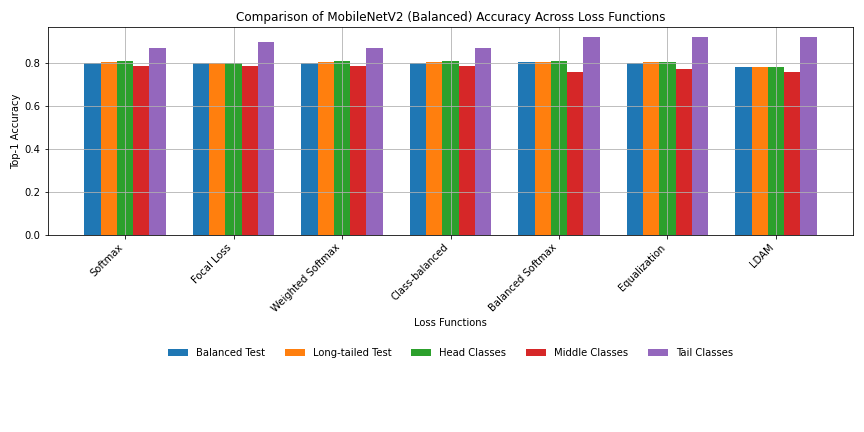
\includegraphics[width=\textwidth]{Images/Plots/mobilenet_bal_loss_comparison.png}
    \caption{Top-1 accuracy comparison of MobileNetV2 trained on the balanced CIFAR-100 across loss functions on different test datasets. The bars represent performance on balanced test data, long-tailed test data, and head, middle, and tail classes.}
    \label{fig:mobilenet_bal_loss_comparison}
\end{figure}

\todo{Comment on \ref{fig:mobilenet_bal_loss_comparison}.}

From Table \ref{tab:mobilenet_bal_acc1_1}, the overall best performance on MobileNetV2 trained with a balanced CIFAR100 training dataset is achieved by Balanced Softmax Loss, which has the highest accuracy on the balanced test dataset (Acc1: 0.8034), as well as on the head (Acc1: 0.8069) and tail (Acc1: 0.9211) classes, with only slightly worse performance on the middle classes in comparison. Among all loss functions, LDAM Loss shows the lowest overall performance on the balanced test set (Acc1: 0.7828) and the long-tailed test set (Acc1: 0.7821), except for its strong performance on tail classes (Acc1: 0.9211). % This highlights LDAM’s specialized focus on tail classes at the cost of performance on head and middle classes.

Softmax Loss, Weighted Softmax Loss, and Class-Balanced Loss yield the same accuracies across all test datasets, likely due to their similarities in loss design  \todo{Refer to background section}.

Balanced Softmax Loss, Equalization Loss, and LDAM Loss exhibit the highest accuracy on tail classes (Acc1: 0.9211). Despite their differing loss designs, this convergence in accuracy suggests that the dataset's tail-class performance may have reached a plateau, possibly due to the inherent characteristics of the tail classes, i.e. either noise or the limited number of samples available per class in the tail \todo{Refer to background section}.

A similar trend is observed in the middle-class accuracy, where Softmax, Focal Loss, Weighted Softmax Loss, and Class-Balanced Loss all achieve identical results (Acc1: 0.7870). Similarly, for head classes, Softmax, Weighted Softmax Loss, Class-Balanced Loss, and Balanced Softmax Loss perform equally well, achieving the highest accuracy (Acc1: 0.8069). % hinting at saturation. This consistency across different loss functions on the balanced dataset could be due to their shared design principles.

% TODO: Compare results to related studies of MobileNetV2 trained on CIFAR100 [table \ref{tab:comparison_mobilenet}]. Mention that the results from MobileNetV2 on the balanced CIFAR100 are okay but not the greatest.




% However, because balanced softmax loss does not yield the same result on both the balanced test set and the long-tailed test set as the other three mentioned, it is likely due to a saturation in the head classes. The softmax loss, weighted softmax loss, and class-balanced loss all yield the same performance across test sets, showing their similiarity in loss design on a balanced training dataset. The best perfoming loss function on the balanced test set is the weighted softmax loss (Acc1: 0.8034), however this is not the best performing loss function on the complete long-tailed dataset, but it has the best accuracy on tail classes (Acc1: 0.9211), and comparable performance on head and tail classes. Except for the performance on tail classes, the overall worst performing loss method is the LDAM loss, with accuracy of 0.7828 on a balanced test set, and 0.7821 on a long-tailed test set. Compared to the baseline, the softmax loss, that has an accuracy of 0.7978 on the balanced test set, and 0.8059 on the long-tailed test set.


% Balanced Softmax Loss, however, stands out due to its differentiated performance across datasets. Unlike Softmax, Weighted Softmax Loss, and Class-Balanced Loss, which yield consistent results across balanced and long-tailed datasets, Balanced Softmax achieves a higher accuracy on tail classes while showing slight variability in overall performance. This suggests that Balanced Softmax is more sensitive to class-specific adjustments, particularly in imbalanced scenarios.


% 
% Compared to the baseline Softmax Loss (balanced: Acc1: 0.7978, long-tailed: Acc1: 0.8059), Balanced Softmax Loss demonstrates slightly better performance on the balanced dataset but shows more variability on the long-tailed dataset, where it achieves comparable results on tail classes but lower performance overall.

\subsubsection{Results from Long-Tailed Training Dataset}

Table \ref{tab:mobilenet_lt_acc1_1} shows the top 1 accuracies for MobileNetV2 on all loss functions.

\begin{table}[H]
    \centering
    \caption{Top-1 accuracy results for MobileNetV2 on the long-tailed dataset across all loss functions.}
    \begin{tabular}{cccccc}
        \toprule
        Loss Function & Balanced & Long-tailed & Head & Middle & Tail \\ 
        \midrule
        Softmax   & 0.5282   & 0.7735 & 0.8341 & 0.5917 & 0.2368 \\
        Focal loss   & 0.5200   & \textbf{0.7745} & \textbf{0.8389} & 0.5917 & 0.1579 \\
        Weighted Softmax loss   & 0.5016   & 0.7231 & 0.7808 & 0.5503 & 0.2105 \\
        Class-balanced loss   & 0.1936   & 0.0913 & 0.0521 & 0.2485 & 0.2632 \\
        Balanced Softmax loss   & \textbf{0.5796}   & 0.7650 & 0.8069 & \textbf{0.6331} & \textbf{0.4211} \\
        Equalization loss   & 0.5310   & 0.7650 & 0.8235 & 0.5917 & 0.2368 \\
        LDAM loss   & 0.4264 & 0.5899 & 0.6137 & 0.5444 & 0.2632 \\
        \bottomrule
    \end{tabular}
    \label{tab:mobilenet_lt_acc1_1}
\end{table}

\begin{figure}[h!]
    \centering
    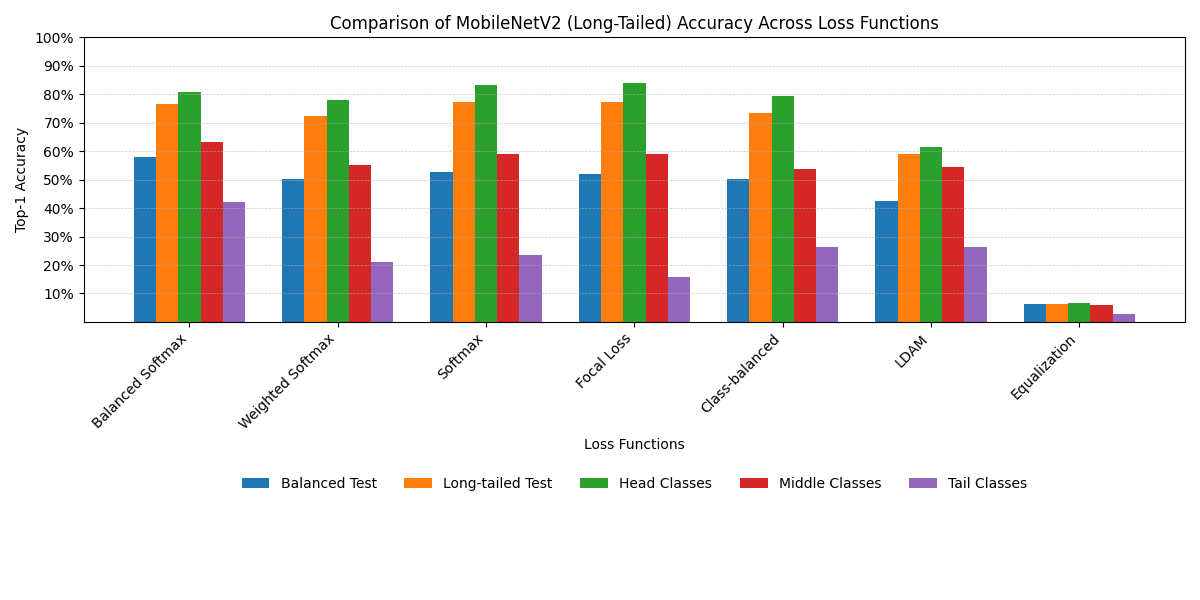
\includegraphics[width=\textwidth]{Images/Plots/mobilenet_lt_loss_comparison.png}
    \caption{Top-1 accuracy comparison of MobileNetV2 trained on the long-tailed CIFAR-100 across loss functions on different test datasets. The bars represent performance on balanced test data, long-tailed test data, and head, middle, and tail classes.}
    \label{fig:mobilenet_lt_loss_comparison}
\end{figure}

\todo{Comment on figure \ref{fig:mobilenet_lt_loss_comparison}.}

From table \ref{tab:mobilenet_lt_acc1_1}, the best overall performance on MobileNetV2 trained with a long-tailed CIFAR100 training dataset is achieved by Balanced Softmax Loss, with the highest accuracy on the balanced test set (Acc1: 0.5796), middle classes (Acc1: 0.6331), and tail classes (Acc1: 0.4211), and with competing accuracies on the long-tailed test dataset (Acc1: 0.7650) and head classes (Acc1: 0.8069), with the highest performance of Focal Loss with top-1 accuracies of 0.7745 and 0.8389, respectively.

The Class-Balanced loss exhibits the least satisfactory accuracies across all test dataset (Balanced: 0.1936, Long-Tailed: 0.0913, Head: 0.0521, Middle: 0.2485), with the only exception at tail classes (Acc1: 0.2632), where the results are comparable to those of other loss designs. This is a contrast to the performance when trained with a balanced CIFAR100 dataset, where the loss design performed within range of the other loss designs, possibly indicating a fault in implementation \todo{investigate implementation}.

Unlike the performance of loss functions trained on the balanced CIFAR100, there are not as many incidents of accuracies of the same value, except for the performance of Softmax Loss, Focal Loss, and Equalization loss on middle classes (Acc1: 0.5917). However, this value is not the highest, as the Balanced Softmax Loss achieves a top-1 accuracy of 0.6331. \todo{explain this.}

\subsubsection{Comparison to Benchmark}
\todo{No benchmark for MobileNetV2 trained on CIFAR-100.}
The paper \textit{BiTAT: Neural Network Binarization
with Task-dependent Aggregated Transformation} by Park et al. tested a MobileNetV2 architecture on CIFAR100 with the highest top 1 accuracy of 73.20 \% .
Link to paper: \url{https://arxiv.org/pdf/2207.01394}

The paper \textit{E$^2$-Train: Training State-of-the-art CNNs with Over
80\% Energy Savings} by Wang et al. reported a top 1 accuracy of 71.91 \% with MobileNetV2 evaluated on CIFAR100.
Link to paper: \url{https://arxiv.org/pdf/1910.13349}

Mine is 80.34 \%. See table \ref{tab:mobilenet_bal_acc1_1}.
% The comparison of my experiment to the original MobileNetV2 trained on the original CIFAR100 dataset.

% Table \ref{tab:comparison_mobilenet} compares the experimental setup and results of MobileNetV2 trained on the CIFAR100 dataset with those reported in Study A3. Key differences include the loss function, optimizer, and data augmentation techniques used.

% While our approach achieves competitive top-1 accuracy on balanced datasets, the performance gap on long-tailed datasets highlights potential areas for improvement in augmentation and learning rate strategies.

% TODO: Move comparisons of results to a seperate section. Keep only the results, put specification in an appendix.

% \begin{table}[H]
%     \centering
%     \begin{tabular}{lp{5cm}p{5cm}}
%         \toprule
%         \textbf{Aspect} & \textbf{Your Experiment} & \textbf{Their Study (A3)} \\ 
%         \midrule
%         Dataset            & CIFAR100 Customized                & CIFAR100                \\
%         Loss Function      & Softmax Cross-Entropy   & Binary Cross-Entropy    \\
%         Epochs             & 90                      & 100                     \\
%         Optimizer          & Adam                    & LAMB                    \\
%         Learning Rate      & Step decay at 30, 60 epochs & Cosine decay from 0.005 or 0.008 \\
%         Augmentation       & Resize (224x224), RandomCrop, Horizontal Flip, Normalize & RandAugment, Mixup, CutMix, Normalize \\
%         Hardware           & 4x NVIDIA TITAN X (Pascal, 12GB) & 4x NVIDIA V100 (32GB) \\
%         Evaluation Metric  & Top-1 Accuracy          & Top-1 Accuracy          \\
%         Top-1 Accuracy     & 79.8 \% & 86.2\%-86.9\%           \\
%         \bottomrule
%     \end{tabular}
%     \caption{Comparison of MobileNetV2 on CIFAR100 with their study (Procedure A3) \cite{wightman2021resnetstrikesbackimproved}.}
%     \label{tab:comparison_mobilenet}
% \end{table}


\subsection{ResNet50V2}

\subsubsection{Results from Balanced Training Dataset}

Table \ref{tab:resnet_bal_acc1_1} show the top 1 accuracies for ResNet50V2 on all loss functions.

\begin{table}[H]
    \centering
    \caption{Evaluation results for ResNet50V2 trained on the custom balanced dataset, showing Acc1.}
    \begin{tabular}{cccccc}
        \toprule
        Loss Function & Balanced & Long-tailed & Head & Middle & Tail \\ 
        \midrule
        Softmax loss   & \textbf{0.8324}  & 0.8421 & 0.8448 & 0.8047 & \textbf{0.9474} \\
        Focal loss   & 0.8310  & 0.8344 & 0.8341 & \textbf{0.8166} & 0.9211 \\
        Weighted Softmax loss   & \textbf{0.8324} & 0.8421 & 0.8448 & 0.8047 & \textbf{0.9474} \\
        Class-balanced loss   &  \textbf{0.8324} & 0.8421 & 0.8448 & 0.8047 & \textbf{0.9474} \\
        Balanced Softmax loss   & 0.8310 & \textbf{0.8430} & \textbf{0.8460} & 0.8107 & 0.9211 \\
        Equalization loss   & 0.8292 & 0.8373 & 0.8412 & 0.7929 & \textbf{0.9474} \\
        LDAM loss   & 0.7990 & 0.7983 & 0.8069 & 0.7337 & 0.8947 \\
        \bottomrule
    \end{tabular}
    \label{tab:resnet_bal_acc1_1}
\end{table}

From table \ref{tab:resnet_bal_acc1_1}, there are three loss designs with the best perfomance on the balanced test dataset, namely Softmax Loss, Weighted Softmax Loss, and Class-Balanced Loss (Acc1: 0.8324). Furthermore, they all yeild the same results across all test dataset due to their cross-entropy architecture for balanced training data. Likewise they yield the best perfomance on the tail classes along with equalization loss (Acc1: 0.9474) \todo{explain}. % possibly due to the low number of samples in the tail classes.

The perfomance of the Balanced Softmax Loss shows excellence on the long-tailed dataset (Acc1: 0.8430) as well as the head classes (Acc1: 0.8460) with competing results on both middle (Acc1: 0.8107) and tail (Acc1: 0.9211) classes.

The worst performance is that of the LDAM loss across all test datasets.

\subsubsection{Results from Long-Tailed Training Dataset}

Table \ref{tab:resnet_lt_acc1_1} show the top 1 accuracies for ResNet50V2 on various loss functions.

\begin{table}[H]
    \centering
    \caption{Evaluation results for ResNet50V2 trained on the long-tailed dataset, showing Acc1.}
    \begin{tabular}{cccccc}
        \toprule
        Loss Function & Balanced & Long-tailed & Head & Middle & Tail \\ 
        \midrule
        Softmax loss   & 0.5522 & \textbf{0.7954} & \textbf{0.8531} & 0.6391 & 0.2105 \\
        Focal loss   & 0.5456 & 0.7935 & 0.8483 & 0.6272 & 0.3158 \\
        Weighted Softmax loss   & 0.4976 & 0.7336 & 0.7915 & 0.5562 & 0.2368 \\
        Class-balanced loss   & 0.2052 & 0.1836 &  0.1445 & 0.3787 & 0.1842 \\
        Balanced Softmax loss   & \textbf{0.5908} & 0.7916 & 0.8270 & \textbf{0.6568} & \textbf{0.6053} \\
        Equalization loss   & 0.5452 & 0.7897 & 0.8389 & 0.6450 & 0.3421 \\
        LDAM loss   & 0.3742 & 0.5937 & 0.6469 & 0.4438 & 0.0789 \\
        \bottomrule
    \end{tabular}
    \label{tab:resnet_lt_acc1_1}
\end{table}


From table \ref{tab:resnet_lt_acc1_1}, the performance of the Balanced Softmax Loss present the best on the balanced dataset (Acc1: 0.5906), middle (Acc1: 0.6568), and tail classes (Acc1: 0.6053) with competing perfomances on the long-tailed datsaet (Acc1: 0.7916) and head classes (Acc1: 0.8270). The best performance on the long-tailed dataset and head classes was presented by the Softmax Loss (Acc1: 0.7954, 0.8531).

Two loss designs are competing for the worst performance with underwhelming results across all test datasets, namely the Class-Balanced loss and the LDAM loss. The LDAM loss achieved an accuracy of 0.0789 on the tail classes, while remaining stable, but unsatisfactory on the rest. The Class-balanced loss with the highest accuracy of 0.3787 across all test datasets has a performance of negligence.

\subsubsection{Comparison to Benchmark}
\todo{No benchmark for ResNet50V2 trained on CIFAR-100. Closest architecture is ResNet50 from the paper \textit{ResNet strikes back: An improved training procedure in timm} \cite{wightman2021resnetstrikesbackimproved}.}

Top 1 accuracy trained on a balanced CIFAR100:
Their: 86.9 \%.
Mine: 83.2 \%.

\todo{Describe differences.}

\subsection{ViT-B/16}

\subsubsection{Results from Balanced Training Dataset}

\begin{table}[H]
    \centering
    \caption{Evaluation results for ViT-B/16 trained on the custom balanced dataset, showing Acc1.}
    \begin{tabular}{cccccc}
        \toprule
        Loss Function & Balanced & Long-tailed & Head & Middle & Tail \\ 
        \midrule
        Softmax loss   & 0.5620 & 0.5671 & 0.5521 & 0.6036 & 0.7368 \\
        Focal loss   & 0.5516 & 0.5538 & 0.5438 & 0.5680 & 0.7105 \\
        Weighted Softmax loss   & 0.5620 & 0.5671 & 0.5521 & 0.6036 & 0.7368 \\
        Class-balanced loss   & 0.5620 & 0.5671 &  0.5521 & 0.6036 & 0.7368 \\
        Balanced Softmax loss   & 0.5628 & 0.5642 & 0.5640 & 0.5325 & 0.7105 \\
        Equalization loss   & 0.5634   & 0.5519 & 0.5462 & 0.5503 & 0.6842 \\
        LDAM loss   & \textbf{0.5906} &  \textbf{0.6013} & \textbf{0.5924} & \textbf{0.6095} & \textbf{0.7632} \\
        \bottomrule
    \end{tabular}
    \label{tab:vit_bal_acc1_1}
\end{table}

From table \ref{tab:vit_bal_acc1_1} it is clear that the loss design with the overall best perfomance on the ViT-B/16 architechture is the LDAM loss. However, the performance of all loss designs across all test datasets are noticably worse than the performance of the other model architectures in this experiment trained with the balanced training dataset. See tables \ref{tab:mobilenet_bal_acc1_1}, \ref{tab:resnet_bal_acc1_1}, and \ref{tab:conv_bal_acc1_1} for reference.  

There is no noticably trend in overall worst performance across loss designs, as all loss function perform within range of each other on all datasets.

\todo{Consider if it make sense to calculate the standard deviation of results within datasets.}  

\subsubsection{Results from Long-Tailed Training Dataset}

\begin{table}[h!]
    \centering
    \caption{Evaluation results for ViT-B/16 trained on the long-tailed dataset, showing Acc1.}
    \begin{tabular}{cccccc}
        \toprule
        Loss Function & Balanced & Long-tailed & Head & Middle & Tail \\ 
        \midrule
        Softmax loss   & 0.2254 & \textbf{0.4367} & \textbf{0.5071} & 0.1775 & 0.0263 \\
        Focal loss   & 0.2210 & 0.4206 & 0.4834 & 0.1953 & 0.0263 \\
        Weighted Softmax loss   & 0.1284 & 0.1760 & 0.1919 & 0.1302 & 0.0263 \\
        Class-balanced loss   & 0.0558 & 0.0076 & 0.0000 & 0.0237 & \textbf{0.1053} \\
        Balanced Softmax loss   & \textbf{0.2460} & 0.4244 & 0.4822 &  \textbf{0.2130} & 0.0789 \\
        Equalization loss   & 0.2168 & 0.4215 & 0.4893 & 0.1716 & 0.0263 \\
        LDAM loss   & 0.1570 & 0.2750 & 0.3140 & 0.1361 & 0.0263 \\
        \bottomrule
    \end{tabular}
    \label{tab:vit_lt_acc1}
\end{table}

From table \ref{tab:vit_lt_acc1}, the best perfomance on the balanced test dataset is accomplshed by th Balanced Softmax loss (Acc1: 0.2460) which also has the best perfomance on middle classes (Acc1: 0.2130), while the Softmax loss achieves the best performance on the long tailed dataset (Acc1: 0.4367) as well as the head classes (0.5071). The best performance on tail classes is achieved by the Class-Balanced loss (Acc1: 0.1053) \todo{check this again}, however this loss design has an underwhelming performance across all other test sets with the lowest achieved perfomance on the head classes with 0.000 accuracy \todo{explain}. 

In all tests, the only loss design achieving a higher accuracy than 50 \% is the Softmax loss on the head classes, meaning that the model underperforms across all loss designs.

\subsubsection{Comparison to Benchmark}
The best result from ViT-B/16 trained with CIFAR100 is obtained in \textit{Perturbated Gradients Updating within Unit Space for Deep Learning} \cite{Tseng_2022} with the best accuracy of 93.95 \%. In comparison, the highest achieved accuracy on a balanced test dataset in this experiment on ViT-B/16 trained with a balanced CIFAR100 was 59.1 \%. See table \ref{tab:vit_bal_acc1_1}. \todo{Compare methods.}
Link to paper: \url{https://arxiv.org/pdf/2110.00199v2}

\todo{Make a table with results.}

% \todo{Move comparisons of results to a seperate section. Keep only the results, put specification in an appendix.}

% \begin{table}[h!]
%     \centering
%     \renewcommand{\arraystretch}{1.2} % Adjust row spacing
%     \setlength{\tabcolsep}{4pt} % Adjust column spacing
%     \begin{tabular}{lp{6cm}p{6cm}}
%         \toprule
%         \textbf{Aspect} & \textbf{Your Experiment} & \textbf{PUGD Results} \\ 
%         \midrule
%         Dataset           & CIFAR100 & CIFAR100 \\
%         Model             & ViT-B/16 pretrained on ImageNet-21K & Multiple models: VGG-16, ResNet-18, DenseNet-121, UPANet-16, and ViT-B/16 \\
%         Pretraining       & ImageNet-21K & ImageNet-1K (for fine-tuned models) \\
%         Optimizer         & Adam & PUGD \\
%         Loss Function     & Softmax Cross-Entropy & Softmax Cross-Entropy \\
%         Epochs            & 90 & 200 (end-to-end); 80–100 (fine-tuning) \\
%         Learning Rate     & Step decay: 0.001 → 0.0001 → 0.00001 & Cosine Annealing: 0.1 (end-to-end); 0.01–0.005 (fine-tuning) \\
%         Augmentation      & Resize (224), RandomCrop, Horizontal Flip, Normalize & Resize (224), RandAugment, Cutout, Normalize \\
%         Top-1 Accuracy    & - & End-to-End: Up to 78.30\% (DenseNet-121); Fine-tuning: ViT-B/16 achieves 93.95\% \\
%         Hardware          & 4x NVIDIA TITAN X (Pascal, 12GB) & RTX-Titan, 32GB RAM, eight-core processor \\
%         \bottomrule
%     \end{tabular}
%     \caption{Comparison of my experiment with PUGD results on CIFAR-100.}
%     \label{tab:comparison3}
% \end{table}


\subsection{ConvNeXt Base}

\subsubsection{Results from balanced Training Dataset}

\begin{table}[h!]
    \centering
    \caption{Evaluation results for ConvNeXt Base trained on the custom balanced dataset, showing Acc1.}
    \begin{tabular}{cccccc}
        \toprule
        Loss Function & Balanced & Long-tailed & Head & Middle & Tail \\ 
        \midrule
        Softmax loss   & 0.8332 & \textbf{0.8535} & \textbf{0.8566} & 0.8166 & \textbf{0.9474} \\
        Focal loss   & 0.8314 & 0.8487 & 0.8507 & 0.8284 & 0.8947 \\
        Weighted Softmax loss   & 0.8332 & \textbf{0.8535} & \textbf{0.8566} &  0.8166 & \textbf{0.9474} \\
        Class-balanced loss   & 0.8332 & \textbf{0.8535} & \textbf{0.8566} & 0.8166 & \textbf{0.9474} \\
        Balanced Softmax loss   & \textbf{0.8364} & 0.8344 & 0.8365 & 0.7988 & \textbf{0.9474} \\
        Equalization loss   & 0.8318 & 0.8468 & 0.8448 & \textbf{0.8343} & \textbf{0.9474} \\
        LDAM loss   & 0.8316 & 0.8373 & 0.8412 & 0.8047 & 0.8947 \\
        \bottomrule
    \end{tabular}
    \label{tab:conv_bal_acc1_1}
\end{table}

From table \ref{tab:conv_bal_acc1_1}, the best performance on the balanced test dataset is achieved by the Balanced Softmax Loss (Acc1: 0.8364), while also achieving the best result on the tail classes (Acc1: 0.9474).

Not surprisingly, the Softmax loss, Weighted Softmax loss, and Class-balanced loss exhibits the same performance across all test dataset, as they were trained with the balanced training dataset, and their designs reduces to the Softmax loss. These three loss function exhibit the best performance on the long-tailed dataset (0.8535), head classes (Acc1: 0.8566) and tail classes (Acc1: 0.9474). The best performance on middle classes is achieved my the Equalization loss (Acc1: 0.8343).

Five out of six loss design achieve the same performance on the tail classes, likely due to saturation causes by the limited number of samples and noise.

\todo{Explain why balanced softmax could achieve higher accuracy in the balanced dataset.}

\subsubsection{Results from Long-Tailed Training Dataset}


\begin{table}[h!]
    \centering
    \caption{Evaluation results for ConvNeXt Basetrained on the long-tailed dataset, showing Acc1.}
    \begin{tabular}{cccccc}
        \toprule
        Loss Function & Balanced & Long-tailed & Head & Middle & Tail \\ 
        \midrule
        Softmax loss   & 0.5972 & \textbf{0.8316} & \textbf{0.8898} & 0.6568 & 0.3158 \\
        Focal loss   & 0.5938 & 0.8145 & 0.8685 & 0.6568 & 0.3158 \\
        Weighted Softmax loss   & 0.4090 & 0.6356 & 0.6848 & 0.4911 & 0.1842 \\
        Class-balanced loss   & 0.0142 & 0.0019 & 0.0000 & 0.0000 & 0.0526 \\
        Balanced Softmax loss   & \textbf{0.6460} & 0.8230 & 0.8685 & 0.6509 & \textbf{0.5789} \\
        Equalization loss   & 0.5956 & 0.8278 & 0.8768 & \textbf{0.6923} & 0.3421 \\
        LDAM loss   & 0.3770 & 0.5956 & 0.6445 & 0.4260 & 0.2632 \\
        \bottomrule
    \end{tabular}
    \label{tab:conv_lt_acc1_1}
\end{table}

From table \ref{tab:conv_lt_acc1_1} the best performance on a balanced test dataset is achived by the Balanced Softmax loss (Acc1: 0.6460), which was the same for the ConvNeXt Base trained with the balanced CIFAR100. See table \ref{tab:conv_bal_acc1_1}. Likewise, the Balanced Softmax loss performs with the highest accuracy on the tail classes (Acc1: 0.5789), far exceeding the second highest performance, achieved by Equalization loss (Acc1: 0.3421). The highest accuracy on the long-tailed dataset (Acc1: 0.8316), as well as the head classes (Acc1: 0.8898), is achieved by the Softmax Loss, while Equalization Loss performs with highest accuracy on middle classes (Acc1: 0.6923). In comparison, the Balanced Softmax loss is third in accuracy on the long-tailed dataset, head classes, as well as middle classes. 

Noticably, both Softmax loss and focal loss performs with equal accuracies on both middle (Acc1: 0.6568) and tail classes (Acc1: 0.3158), but not elsewhere. \todo{give a reason why that might be.}

The worst performance is achieved by the Class-Balanced loss, with accuracies far below the second worst performances. The Class-balanced loss should be disregarded for training with a long-tailed dataset, as it is most likely a fault in implementation. \todo{investigate this and return to this conclusion.}


\subsubsection{Comparison to Benchmark}
\todo{No benchmark found for ConvNeXt Base trained with CIFAR100.}
Closest is \textit{Conv2NeXt: Reconsidering Conv NeXt Network Design for Image Recognition} by Feng et al. with top 1 accuracy of 83.82 \% in CIFAR-100. Mine is 83.64 \%.
Link: \url{https://ieeexplore.ieee.org/document/10072172}

\section{Comparison of Models}
Analyze how different models impact performance.
Use visualizations to compare results.
Discuss strengths and weaknesses of each model.

\begin{figure}[h!]
    \centering
    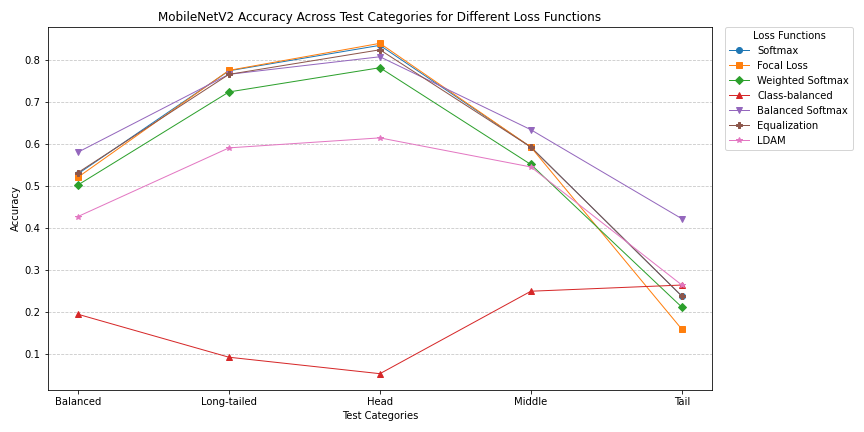
\includegraphics[width=\textwidth]{Images/Plots/mobilenet_lt_loss_comparison_line.png}
    \caption{MobileNetV2 top 1 accuracy across test categories (Balanced, Long-tailed, Head, Middle, Tail) for different loss functions.}
    \label{fig:mobilenet_bal_loss_comparison_line}
\end{figure}

\begin{figure}[h!]
    \centering
    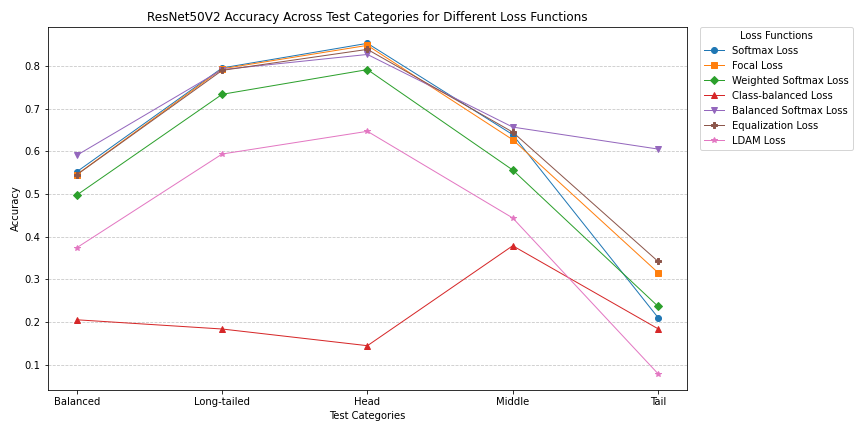
\includegraphics[width=\textwidth]{Images/Plots/resnet_lt_loss_comparison_line.png}
    \caption{ResNet50V2 top 1 accuracy across test categories (Balanced, Long-tailed, Head, Middle, Tail) for different loss functions.}
    \label{fig:resnet_bal_loss_comparison_line}
\end{figure}

\begin{figure}[h!]
    \centering
    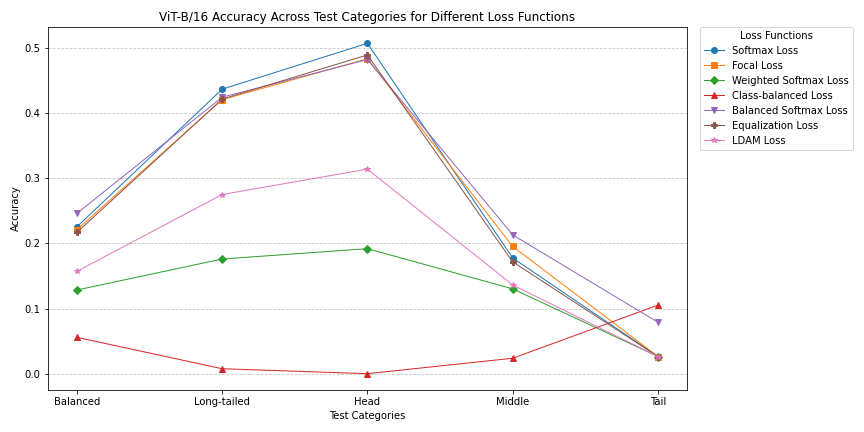
\includegraphics[width=\textwidth]{Images/Plots/vit_lt_loss_comparison_line.png}
    \caption{ViT-B/16 top 1 accuracy across test categories (Balanced, Long-tailed, Head, Middle, Tail) for different loss functions.}
    \label{fig:vit_bal_loss_comparison_line}
\end{figure}

\begin{figure}[h!]
    \centering
    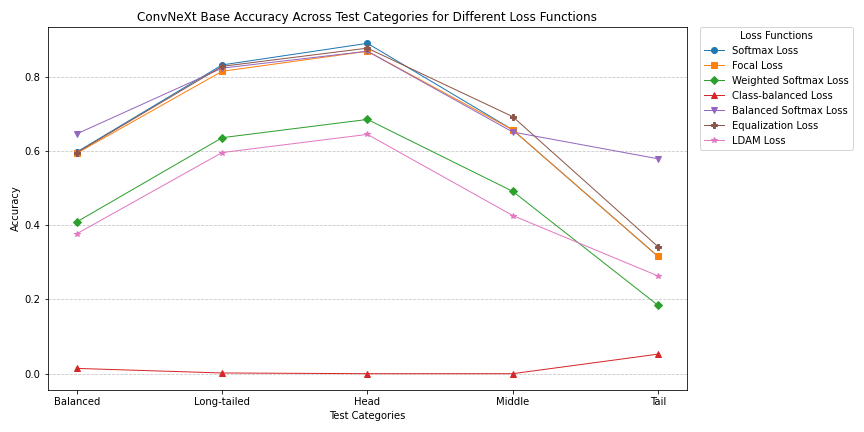
\includegraphics[width=\textwidth]{Images/Plots/convnext_lt_loss_comparison_line.png}
    \caption{ConvNeXt Base top 1 accuracy across test categories (Balanced, Long-tailed, Head, Middle, Tail) for different loss functions.}
    \label{fig:conv_bal_loss_comparison_line}
\end{figure}

\subsubsection{Mean and Standard Deviation}

\todo{Make a table for the mean and standard deviations.}

The plots on figures \ref{fig:mean_loss_comparison_line} and \ref{fig:mean_loss_comparison_line_noCB} compares the performance of the models MobileNetV2, ResNet50V2, ViT-B/16, and ConvNeXt Base across the evaluation categories: balanced, long-tailed, head, middle, and tail. Each model is slightly offset along the x-axis to avoid overlap. The mean and standard deviation in figure \ref{fig:mean_loss_comparison_line} include the Class-Balanced Loss while figure \ref{fig:mean_loss_comparison_line_noCB} does not.

Each point represents the mean accuracy of a model for a specific category and the bars represent the standard deviation. A model with higher mean accuracy is performing better in that category, and a smoother or higher line indicates consistent performance across all categories.

The error bars show the variability in accuracy across different loss functions for each model and category. A longer error bar means the performance is less consistent and the performance is more dependent on the chosen loss function, while shorter error bars indicate consistant performance.

The plot in figure \ref{fig:mean_loss_comparison_line_noCB} shows that the model with the best average performance on tail classes is the ConvNeXt Base architecture, while also showing a strong performance in other categories. 

MobileNetV2 is the least dependent on loss functions, exhibiting the smallest standard deviation, while the ResNet50V2 architecture, compared with figures \ref{fig:resnet_bal_loss_comparison_line} and \ref{fig:conv_bal_loss_comparison_line}, is the most dependent on loss functions when exhibiting tail performance, as the Balanced Softmax Loss outperforms the remaining loss functions, as seen in figure \ref{fig:resnet_bal_loss_comparison_line} and table \ref{tab:resnet_lt_acc1_1}.

The model exhibiting the worst performance is the ViT-B/16 with a significant lower mean than the other three models.

\begin{figure}[h!]
    \centering
    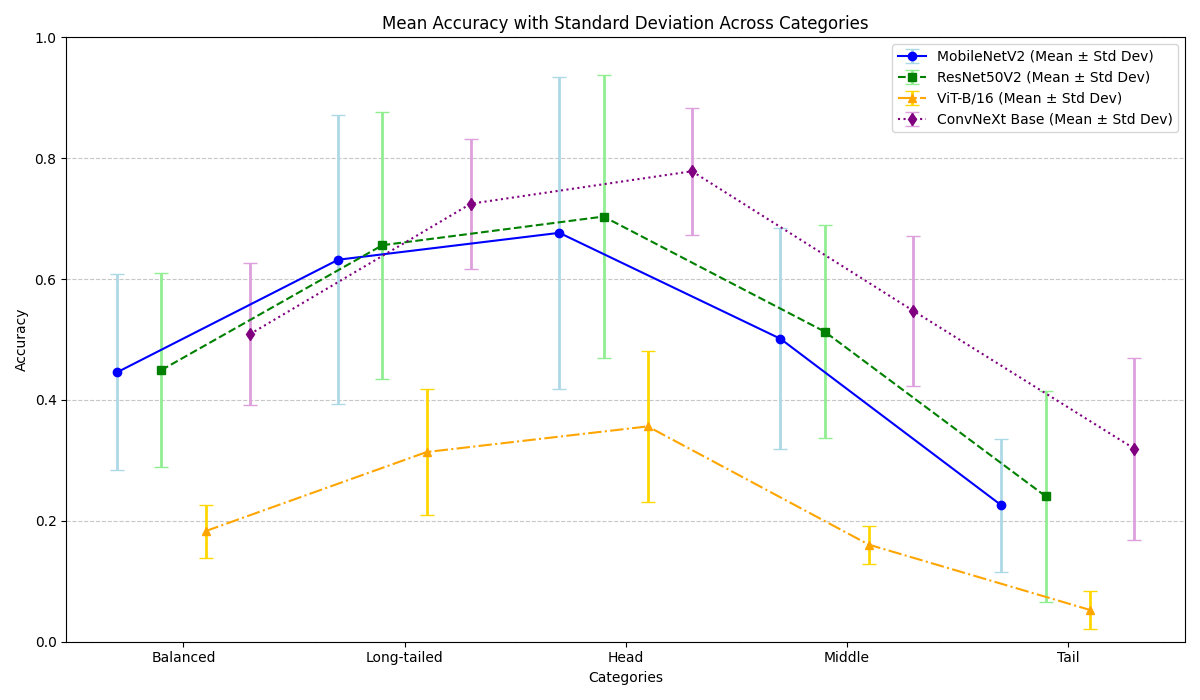
\includegraphics[width=\textwidth]{Images/Plots/mean_loss_comparison.png}
    \caption{Mean Accuracy with Standard Deviation Across Categories for MobileNetV2, ResNet50V2, ViT-B/16, and ConvNeXt Base.}
    \label{fig:mean_loss_comparison_line}
\end{figure}

\begin{figure}[h!]
    \centering
    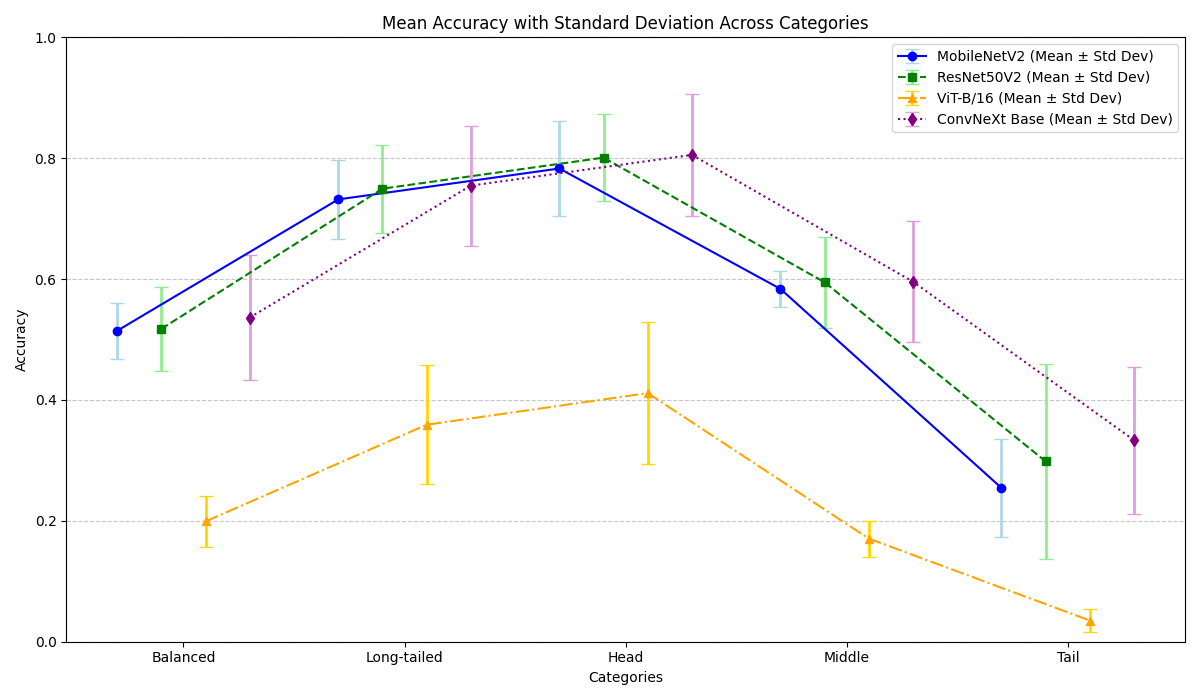
\includegraphics[width=\textwidth]{Images/Plots/mean_loss_comparison_noCB.png}
    \caption{Mean Accuracy with Standard Deviation Across Categories for MobileNetV2, ResNet50V2, ViT-B/16, and ConvNeXt Base without Class-Balanced Loss.}
    \label{fig:mean_loss_comparison_line_noCB}
\end{figure}


\todo{Comparison of overall model performance. Potentially statistical analysis, e.g. ANOVA, Tukey's HSD.}

\section{Comparison of Loss Functions}
\todo{Analyze how different loss functions impact performance.} 

From figure \ref{fig:loss_comparison} it can be seen that the Balanced Softmax Loss has a better average perfomance on tail classes, while also displaying the smoothest variation across evaluation categories, ignoring the Class-Balanced loss. However, the standard deviation suggests that the perfomance of the Balanced Softmax Loss depend on the model architecture.

\begin{figure}[h!]
    \centering
    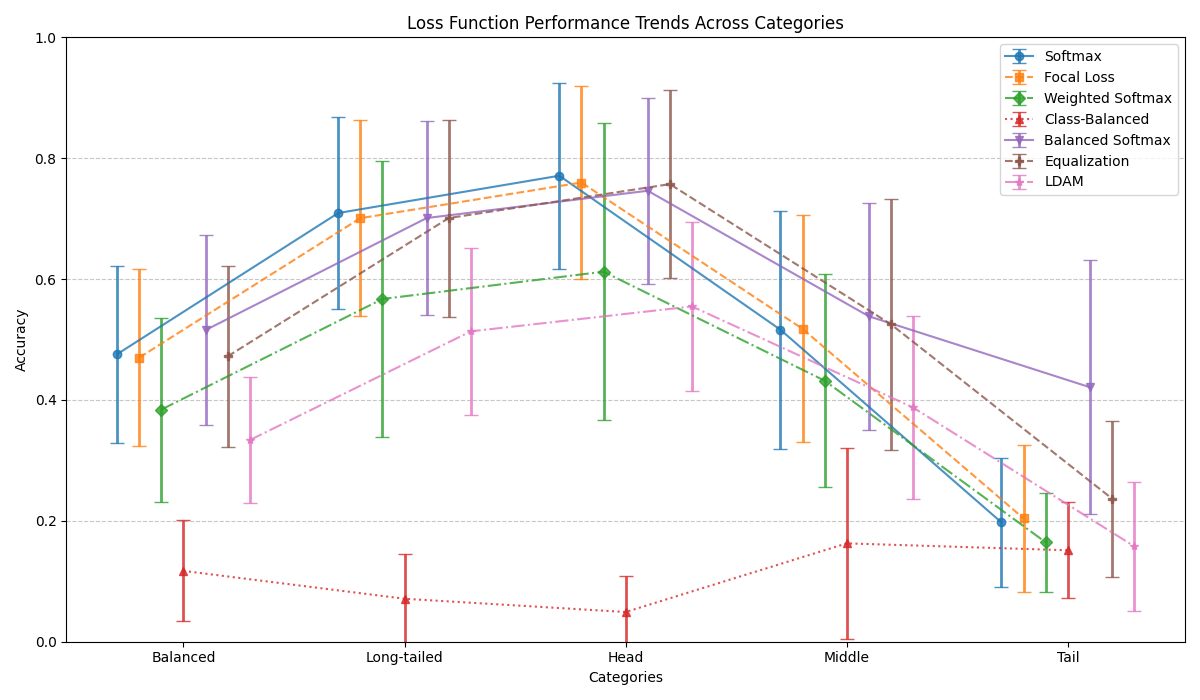
\includegraphics[width=\textwidth]{Images/Plots/loss_comparison.png}
    \caption{Performance trends of different loss functions across evaluation categories. Error bars indicate the standard deviation of accuracy across models, highlighting variability in performance for each loss function.}
    \label{fig:loss_comparison}
\end{figure}



\section{Comparison with Baselines}
Compare the results to the softmax cross-entropy loss, and compare to the model trained with balanced dataset.

\section{Comparison with Benchmarks}
The results are compared to the best published results for MobileNetV2, ResNet50V2, ViT-B/16 and ConvNeXt Base on CIFAR-100.

To contextualize the performance of models, the results are compared against the best posted results for the same architecture on CIFAR-100, reported by Author/Source.

\todo{Move benchmark results into a table.}

% Highlight Key Differences
% If there are differences in training conditions (e.g., data augmentation, optimization strategies, or hardware), acknowledge them:
% "It is important to note that while our setup involves an imbalanced CIFAR-100 dataset, the benchmark results were obtained on a balanced dataset."
% "Our experiments use an Adam optimizer, whereas [Source] employed SGD with momentum."

% \section{Qualitative Results}
% Include if time.
% Provide examples of correctly and incorrectly classified samples, especially for tail classes.
% Include visualizations or images of difficult cases to highlight challenges in tail-class prediction.

\section{Summary and Discussion}
Things for discussion:

\begin{itemize}
    \item Why is the performance on tail classes better than the performance on head and middle classes for the balanced training data, and what could it mean for the results on the long-tail training data?
    \item Running multiple of the same training to check for variance. What could this tell us in terms of statistical significance?
    \item The LDAM should be run with DRW as well. Compare to articles that run both LDAM and LDAM-DRW.
    \item Including or omitting the Class-Balanced Loss.
    \item Discuss why the ViT-B/16 model underperforms but shows excellent performance in other studies.
\end{itemize}

Balanced Softmax Loss emerged as the most effective loss function for addressing the lack of samples in tail classes, consistently achieving the highest accuracy on these classes across all tested models. This result highlights its strength in re-weighting logits to account for imbalanced datasets, particularly for tail classes, where traditional loss functions often falter. The synergy between Balanced Softmax and certain architectures, such as ConvNeXt Base, was especially notable, suggesting that specific combinations of models and loss functions can yield superior performance.

However, this improvement in tail-class accuracy often came with trade-offs. For example, while ResNet50V2 achieved a top-1 accuracy of 0.6053 on tail classes using Balanced Softmax, its head-class accuracy (0.8270) lagged behind ConvNeXt Base (0.8685). This trade-off underscores the challenge of optimizing for both head and tail classes simultaneously and indicates that Balanced Softmax prioritizes tail-class adjustments at the expense of head-class performance.

Class-Balanced Loss, in contrast, consistently underperformed across all models and datasets, raising questions about its suitability for highly imbalanced scenarios. The discrepancy between its intended purpose and observed results suggests possible issues with its weighting strategy or implementation. Further investigation is necessary to understand these limitations and determine whether its performance can be improved.

Notably, the ViT-B/16 architecture underperformed significantly across all loss functions and datasets, with an overall accuracy of 59.06\% compared to its benchmark of 93.95\%. This gap suggests that Vision Transformers, despite their success in other contexts, may require more data, longer training, or additional fine-tuning to handle imbalanced datasets effectively. The results indicate that ViT-B/16's default configuration may not be well-suited for long-tailed datasets without further optimization.

While Balanced Softmax stood out as the most robust loss function overall, statistical validation is required to confirm the significance of these findings, particularly when comparing closely performing configurations. For instance, the performance gap between Balanced Softmax and Softmax Loss on middle classes or long-tailed datasets could reflect inherent dataset characteristics rather than the superiority of the loss function alone.

Overall, these findings emphasize the importance of aligning loss functions with both dataset characteristics and model architectures to address the unique challenges of long-tailed learning. They also highlight the need for a nuanced approach that balances improvements in tail-class accuracy with minimal trade-offs in head-class and overall performance.

\chapter{Conclusion and Future Work}
% Chapter 6: Conclusion and Future Work

The findings from the experiments conducted in this thesis underlines the difficulty of achieving strong performances with deep long-tailed learning. Specifically, the results emphasizes the importance of thoughtfully combining model architectures, loss design, and choice of configurations. Among the evaluated approaches, the Balanced Softmax Loss consistently achieved the best performance on tail classes, while maintaining a comparable performance on other categories across multiple CNN backbones. In contrast, Class-Balanced Loss underperformed across all models and categories, suggesting a fault in implementation \todo{investigate}. Likewise, ViT-B/16's performance gap from both CNN-based architectures and its own benchmark imply that vision transformer architectures may require extensive adaptations to reach their full potential.  

\section{Revisiting the Goals of the Thesis}
In revisiting the goals of this thesis, it has become clear that the investigation of the deep long-tailed learning technique \emph{Class Re-Balancing} has yielded valuable insight. The findings included that performance on tail classes often comes with a trade-off in performance on head classes. Similarly, adequate performances on all classes was often attributed to the performance on head classes and not inherently on tail classes, although the Balanced Softmax Loss convincingly overcame this challenge across CNN-based architectures. This aligns with the goal of investigating the ability of deep long-tailed learning techniques to maintain overall accuracy. 

Secondly, the evaluations of different model architectures, namely the CNN-based and Vision Transformers, in combination with different class re-balancing designs has revealed that model design has an effect on the performance of long-tailed learning, and that the MobileNetV2 architecture exhibits greater robustnes against choice of loss design than other architectues evaluated in this thesis. 

Finally, these findings contribute to a more comprehensive understanding of what to consider when training a deep network with long-tailed data, and, in doing so, serves as a guide to deep learning practitioners seeking more informed choices when encountered with a long-tailed problem.

\section{Future Work}
Future investigation would benefit from evaluating experiments with larger datasets, such as ImageNet or iNaturalist to gain more insight into the performance of models and long-tailed techniques. Additionally, training ViT-B/16 on larger datasets while carefully considering its configurations could prove its full potential. Furthermore, evaluating the LDAM including the DRW and, potentially, combined with other loss functions on CIFAR-100-LT could reveal under which conditions tail-class performance is maximized. Finally, other techniques, such as re-sampling in combination with class re-balancing, should be explored.

% References
\printbibliography[heading=bibintoc]


% Appendices
\begin{appendices}
%\chapter{Results} % Results, code, etc.
Tables of the results from training.


\section{MobileNetV2}
\textit{MobileNetV2 trained on custom balanced dataset and imbalanced dataset on different loss functions.}\\

Table \ref{tab:mobilenet_bal_acc1} show the top 1 accuracies for MobileNetV2 on various loss functions. Table \ref{tab:mobilenet_bal_results} show the loss, top 1 accuracy, and F1 score.\\
Table \ref{tab:mobilenet_lt_acc1} show the top 1 accuracies for MobileNetV2 on various loss functions. Table \ref{tab:mobilenet_lt_results} show the loss, top 1 accuracy, and F1 score. 

\begin{table}[H]
    \centering
    \begin{tabular}{cccccc}
        \toprule
        Loss Function & Balanced & Long-tailed & Head & Middle & Tail \\ 
        \midrule
        Softmax   & 0.7978   & 0.8059 & 0.8069 & 0.7870 & 0.8684 \\
        Focal loss   & 0.8014   & 0.8011 & 0.7998 4 & 0.7870 & 0.8947 \\
        Weighted Softmax loss   & 0.7978   & 0.8059 & 0.8069 & 0.7870 & 0.8684 \\
        Class-balanced loss   & 0.7978   & 0.8059 & 0.8069 & 0.7870 & 0.8684 \\
        Balanced Softmax loss   & 0.8034  & 0.8030 & 0.8069 & 0.7574 & 0.9211 \\
        Equalization loss   & 0.7994   & 0.8040 & 0.8057 & 0.7692 & 0.9211 \\
        LDAM loss   &  0.7828   & 0.7821 & 0.7808 & 0.7574 & 0.9211 \\
        \bottomrule
    \end{tabular}
    \caption{Evaluation results for MobileNetV2 trained on the custom balanced dataset, showing Acc1.}
    \label{tab:mobilenet_bal_acc1}
\end{table}

\begin{table}[H]
    \centering
    \resizebox{\textwidth}{!}{ % Scale to text width
        \begin{tabular}{c|ccc|ccc|ccc|ccc|ccc}
            \toprule
            \multirow{2}{*}{Loss Function} & \multicolumn{3}{c|}{Balanced} & \multicolumn{3}{c|}{Long-tailed} & \multicolumn{3}{c|}{Head} & \multicolumn{3}{c|}{Middle} & \multicolumn{3}{c}{Tail} \\ 
            \cmidrule(lr){2-4} \cmidrule(lr){5-7} \cmidrule(lr){8-10} \cmidrule(lr){11-13} \cmidrule(lr){14-16}
            & Loss & Acc1 & F1 & Loss & Acc1 & F1 & Loss & Acc1 & F1 & Loss & Acc1 & F1 & Loss & Acc1 & F1 \\ 
            \midrule
            Softmax & 1.1455 & 0.7978 & 0.7967 & 1.1415 & 0.8059 & 0.8208 & 1.1208 & 0.8069 & 0.8587 & 1.3060 & 0.7870 & 0.8368 & 0.8690 & 0.8684 & 0.8684 \\
            Focal Loss & 0.6765 & 0.8014 & 0.8001 & 0.7063 & 0.8011 & 0.8175 & 0.7005 & 0.7998 & 0.8531 & 0.8028 & 0.7870 & 0.8293 & 0.4055 & 0.8947 & 0.8860 \\
            Weighted Softmax & 1.1455 & 0.7978 & 0.7967 & 1.1415 & 0.8059 & 0.8208 & 1.1208 & 0.8069 & 0.8587 & 1.3060 & 0.7870 & 0.8368 & 0.8690 & 0.8684 & 0.8684 \\
            Class-balanced & 1.1455 & 0.7978 & 0.7967 & 1.1415 & 0.8059 & 0.8208 & 1.1208 & 0.8069 & 0.8587 & 1.3060 & 0.7870 & 0.8368 & 0.8690 & 0.8684 & 0.8684 \\
            Balanced Softmax & 1.1289 & 0.8034 & 0.8011 & 1.1848 & 0.8030 & 0.8145 & 1.1469 & 0.8069 & 0.8553 & 1.4407 & 0.7574 & 0.8123 & 0.8872 & 0.9211 & 0.9298 \\
            Equalization & 0.9992 & 0.7994 & 0.7983 & 1.0385 & 0.8040 & 0.8192 & 1.0118 & 0.8057 & 0.8564 & 1.2539 & 0.7692 & 0.8213 & 0.6035 & 0.9211 & 0.9211 \\
            LDAM & 13.8126 &  0.7828 & 0.7817 & 13.5566 & 0.7821 & 0.7955 & 13.6884 & 0.7808 & 0.8325 & 14.7496 & 0.7574 & 0.8016 & 5.3231 & 0.9211 & 0.9035 \\
            \bottomrule
        \end{tabular}
    }
    \caption{Evaluation results for MobileNetV2 trained on the custom balanced dataset, showing Loss, Acc1, and F1 scores for each dataset split.}
    \label{tab:mobilenet_bal_results}
\end{table}


\begin{table}[H]
    \centering
    \begin{tabular}{cccccc}
        \toprule
        Loss Function & Balanced & Long-tailed & Head & Middle & Tail \\ 
        \midrule
        Softmax   & 0.5282   & 0.7735 & 0.8341 & 0.5917 & 0.2368 \\
        Focal loss   & 0.5200   & 0.7745 & 0.8389 & 0.5917 & 0.1579 \\
        Weighted Softmax loss   & 0.5016   & 0.7231 & 0.7808 & 0.5503 & 0.2105 \\
        Class-balanced loss   & 0.1936   & 0.0913 & 0.0521 & 0.2485 & 0.2632 \\
        Balanced Softmax loss   & 0.5796   & 0.7650 & 0.8069 & 0.6331 & 0.4211 \\
        Equalization loss   & 0.5310   & 0.7650 & 0.8235 & 0.5917 & 0.2368 \\
        LDAM loss   & 0.4264 & 0.5899 & 0.6137 & 0.5444 & 0.2632 \\
        \bottomrule
    \end{tabular}
    \caption{Evaluation results for MobileNetV2 trained on the long-tailed dataset showing Acc1.}
    \label{tab:mobilenet_lt_acc1}
\end{table}

\begin{table}[H]
    \centering
    \resizebox{\textwidth}{!}{ % Scale to text width
        \begin{tabular}{c|ccc|ccc|ccc|ccc|ccc}
            \toprule
            \multirow{2}{*}{Loss Function} & \multicolumn{3}{c|}{Balanced} & \multicolumn{3}{c|}{Long-tailed} & \multicolumn{3}{c|}{Head} & \multicolumn{3}{c|}{Middle} & \multicolumn{3}{c}{Tail} \\ 
            \cmidrule(lr){2-4} \cmidrule(lr){5-7} \cmidrule(lr){8-10} \cmidrule(lr){11-13} \cmidrule(lr){14-16}
            & Loss & Acc1 & F1 & Loss & Acc1 & F1 & Loss & Acc1 & F1 & Loss & Acc1 & F1 & Loss & Acc1 & F1 \\ 
            \midrule
            Softmax & 3.2503 & 0.5282 & 0.4884 & 1.2212 & 0.7735 & 0.7578 & 0.8136 & 0.8341 & 0.8492 & 2.4604 & 0.5917 & 0.6444 & 4.7629 & 0.2368 & 0.2544 \\
            Focal Loss & 2.3526 & 0.5200 & 0.4818 & 0.8022 & 0.7745 & 0.7602 & 0.5177 & 0.8389 & 0.8528 & 1.5864 & 0.5917 & 0.6625 & 3.6343 & 0.1579 & 0.1667 \\
            Weighted Softmax & 3.1412 & 0.5016 & 0.4690 & 1.2817 & 0.7231 & 0.7104 & 0.8786 & 0.7808 & 0.8015 & 2.3365 & 0.5503 & 0.6213 & 5.1836 & 0.2105 & 0.1912 \\
            Class-balanced & 4.3308 & 0.1936 & 0.1751 & 4.2181 & 0.0913 & 0.0854 & 4.4197 & 0.0521 & 0.0795 & 2.8788 & 0.2485 & 0.2767 & 6.3575 & 0.2632 & 0.2368 \\
            Balanced Softmax & 3.1185 & 0.5796 & 0.5572 & 1.1630 & 0.7650 & 0.7685 & 0.7989 & 0.8069 & 0.8422 & 2.1612 & 0.6331 & 0.6872 & 4.8108 & 0.4211 & 0.4123 \\
            Equalization & 3.0593 & 0.5310 & 0.4911 & 1.1563 & 0.7650 & 0.7499 & 0.7241 & 0.8235 & 0.8398 & 2.4487 & 0.5917 & 0.6524 & 4.9284 & 0.2368 & 0.2544 \\
            LDAM & 21.4896 & 0.4264 & 0.3980 & 7.9893 & 0.5899 & 0.5909 & 5.6756 & 0.6137 & 0.6581 & 10.3379 & 0.5444 & 0.6121 & 49.1197 & 0.2632 & 0.2895 \\
            \bottomrule
        \end{tabular}
    }
    \caption{Evaluation results for MobileNetV2 trained on the long-tailed dataset, showing Loss, Acc1, and F1 scores for each dataset split.}
    \label{tab:mobilenet_lt_results}
\end{table}




\section{ResNet50V2}
\textit{ResNet50V2 trained on custom balanced dataset and imbalanced dataset on different loss functions.}\\

Table \ref{tab:resnet_bal_acc1} show the top 1 accuracies for ResNet50V2 on various loss functions. Table \ref{tab:resnet_bal_results} show the loss, top 1 accuracy, and F1 score.\\

Table \ref{tab:resnet_lt_acc1} show the top 1 accuracies for ResNet50V2 on various loss functions. Table \ref{tab:resnet_lt_results} show the loss, top 1 accuracy, and F1 score. 

\begin{table}[H]
    \centering
    \begin{tabular}{cccccc}
        \toprule
        Loss Function & Balanced & Long-tailed & Head & Middle & Tail \\ 
        \midrule
        Softmax loss   & 0.8324  & 0.8421 & 0.8448 & 0.8047 & 0.9474 \\
        Focal loss   & 0.8310  & 0.8344 & 0.8341 & 0.8166 & 0.9211 \\
        Weighted Softmax loss   & 0.8324 & 0.8421 & 0.8448 & 0.8047 & 0.9474 \\
        Class-balanced loss   &  0.8324 & 0.8421 & 0.8448 & 0.8047 & 0.9474 \\
        Balanced Softmax loss   & 0.8310 & 0.8430 & 0.8460 & 0.8107 & 0.9211 \\
        Equalization loss   & 0.8292 & 0.8373 & 0.8412 & 0.7929 & 0.9474 \\
        LDAM loss   & 0.7990 & 0.7983 & 0.8069 & 0.7337 & 0.8947 \\
        \bottomrule
    \end{tabular}
    \caption{Evaluation results for ResNet50V2 trained on the custom balanced dataset, showing Acc1.}
    \label{tab:resnet_bal_acc1}
\end{table}

\begin{table}[H]
    \centering
    \resizebox{\textwidth}{!}{ % Scale to text width
        \begin{tabular}{c|ccc|ccc|ccc|ccc|ccc}
            \toprule
            \multirow{2}{*}{Loss Function} & \multicolumn{3}{c|}{Balanced} & \multicolumn{3}{c|}{Long-tailed} & \multicolumn{3}{c|}{Head} & \multicolumn{3}{c|}{Middle} & \multicolumn{3}{c}{Tail} \\ 
            \cmidrule(lr){2-4} \cmidrule(lr){5-7} \cmidrule(lr){8-10} \cmidrule(lr){11-13} \cmidrule(lr){14-16}
            & Loss & Acc1 & F1 & Loss & Acc1 & F1 & Loss & Acc1 & F1 & Loss & Acc1 & F1 & Loss & Acc1 & F1 \\ 
            \midrule
            Softmax & 0.9823 & 0.8324 & 0.8310 & 0.9874 & 0.8421 & 0.8520 & 0.9917 & 0.8448 & 0.8860 & 1.0934 & 0.8047 & 0.8467 & 0.4205 & 0.9474 & 0.9386 \\
            Focal Loss & 0.5627 & 0.8310 & 0.8300 & 0.5578 & 0.8344 & 0.8474 & 0.5555 & 0.8341 & 0.8788 & 0.6294 & 0.8166 & 0.8607 & 0.2920 & 0.9211 & 0.9123 \\
            Weighted Softmax & 0.9823 & 0.8324 & 0.8310 & 0.9874 & 0.8421 & 0.8520 & 0.9917 & 0.8448 & 0.8860 & 1.0934 & 0.8047 & 0.8467 & 0.4205 & 0.9474 & 0.9386 \\
            Class-balanced & 0.9823 &  0.8324 & 0.8310 & 0.9874 & 0.8421 & 0.8520 & 0.9917 & 0.8448 & 0.8860 & 1.0934 & 0.8047 & 0.8467 & 0.4205 & 0.9474 & 0.9386 \\
            Balanced Softmax & 1.0198 & 0.8310 & 0.8301 & 0.9689 & 0.8430 & 0.8549 & 0.9601 & 0.8460 & 0.8893 & 1.1309 & 0.8107 & 0.8539 & 0.4440 & 0.9211 & 0.9123 \\
            Equalization & 0.8795 & 0.8292 & 0.8279 & 0.9079 & 0.8373 & 0.8495 & 0.8888 & 0.8412 & 0.8877 & 1.1374 & 0.7929 & 0.8453 & 0.2495 & 0.9474 & 0.9386 \\
            LDAM & 9.8339 & 0.7990 & 0.7979 & 10.1092 & 0.7983 & 0.8119 & 9.8723 & 0.8069 & 0.8596 & 12.5229 & 0.7337 & 0.7823 & 4.6362 & 0.8947 & 0.8772 \\
            \bottomrule
        \end{tabular}
    }
    \caption{Evaluation results for ResNet50V2 trained on the custom balanced dataset, showing Loss, Acc1, and F1 scores for each dataset split.}
    \label{tab:resnet_bal_results}
\end{table}



\begin{table}[H]
    \centering
    \begin{tabular}{cccccc}
        \toprule
        Loss Function & Balanced & Long-tailed & Head & Middle & Tail \\ 
        \midrule
        Softmax loss   & 0.5522 & 0.7954 & 0.8531 & 0.6391 & 0.2105 \\
        Focal loss   & 0.5456 & 0.7935 & 0.8483 & 0.6272 & 0.3158 \\
        Weighted Softmax loss   & 0.4976 & 0.7336 & 0.7915 & 0.5562 & 0.2368 \\
        Class-balanced loss   & 0.2052 & 0.1836 &  0.1445 & 0.3787 & 0.1842 \\
        Balanced Softmax loss   & 0.5908 & 0.7916 & 0.8270 & 0.6568 & 0.6053 \\
        Equalization loss   & 0.5452 & 0.7897 & 0.8389 & 0.6450 & 0.3421 \\
        LDAM loss   & 0.3742 & 0.5937 & 0.6469 & 0.4438 & 0.0789 \\
        \bottomrule
    \end{tabular}
    \caption{Evaluation results for ResNet50V2 trained on the long-tailed dataset, showing Acc1.}
    \label{tab:resnet_lt_acc1}
\end{table}

\begin{table}[H]
    \centering
    \resizebox{\textwidth}{!}{ % Scale to text width
        \begin{tabular}{c|ccc|ccc|ccc|ccc|ccc}
            \toprule
            \multirow{2}{*}{Loss Function} & \multicolumn{3}{c|}{Balanced} & \multicolumn{3}{c|}{Long-tailed} & \multicolumn{3}{c|}{Head} & \multicolumn{3}{c|}{Middle} & \multicolumn{3}{c}{Tail} \\ 
            \cmidrule(lr){2-4} \cmidrule(lr){5-7} \cmidrule(lr){8-10} \cmidrule(lr){11-13} \cmidrule(lr){14-16}
            & Loss & Acc1 & F1 & Loss & Acc1 & F1 & Loss & Acc1 & F1 & Loss & Acc1 & F1 & Loss & Acc1 & F1 \\ 
            \midrule
            Softmax & 3.0907 & 0.5522 & 0.5138 & 1.0524 & 0.7954 & 0.7798 & 0.6888 & 0.8531 & 0.8654 & 2.0330 & 0.6391 & 0.6996 & 4.7658 & 0.2105 & 0.2018 \\
            Focal Loss & 2.0718 & 0.5456 & 0.5089 & 0.6284 & 0.7935 & 0.7789 & 0.3983 & 0.8483 & 0.8583 & 1.3258 & 0.6272 & 0.7054 & 2.6364 & 0.3158 & 0.3158 \\
            Weighted Softmax & 3.7904 & 0.4976 & 0.4591 & 1.3481 & 0.7336 & 0.7198 & 0.8630 & 0.7915 & 0.8098 & 2.2625 & 0.5562 & 0.6209 & 6.9808 & 0.2368 & 0.2456 \\
            Class-balanced & 4.5887 & 0.2052 & 0.1928 & 3.7422 & 0.1836 & 0.1932 & 3.7880 &  0.1445 & 0.2045 & 2.4884 & 0.3787 & 0.4138 & 8.3052 & 0.1842 & 0.1737 \\
            Balanced Softmax & 3.1081 & 0.5908 & 0.5654 & 1.0452 & 0.7916 & 0.7895 & 0.6873 & 0.8270 & 0.8602 & 2.3422 & 0.6568 & 0.7135 & 3.2275 & 0.6053 & 0.5965 \\
            Equalization & 3.0166 & 0.5452 & 0.5071 & 1.0315 & 0.7897 & 0.7756 & 0.7418 & 0.8389 & 0.8511 & 1.8754 & 0.6450 & 0.7061 & 3.6342 & 0.3421 & 0.3509 \\
            LDAM & 22.7933 & 0.3742 & 0.3337 & 8.2056 & 0.5937 & 0.5784 & 5.3320 & 0.6469 & 0.6680 & 12.3074 & 0.4438 & 0.5450 & 53.4080 & 0.0789 & 0.0789 \\
            \bottomrule
        \end{tabular}
    }
    \caption{Evaluation results for ResNet50V2 trained on the long-tailed dataset, showing Loss, Acc1, and F1 scores for each dataset split.}
    \label{tab:resnet_lt_results}
\end{table}


\section{ViT-B/16}
\textit{ViT-B/16 trained on custom balanced dataset and imbalanced dataset on different loss functions.}\\


Table \ref{tab:vit_bal_acc1} show the top 1 accuracies for ViT-B/16 on various loss functions. Table \ref{tab:vit_bal_results} show the loss, top 1 accuracy, and F1 score.\\

Table \ref{tab:vil_lt_acc1} show the top 1 accuracies for ViT-B/16 on various loss functions. Table \ref{tab:vit_lt_results} show the loss, top 1 accuracy, and F1 score.

\begin{table}[H]
    \centering
    \begin{tabular}{cccccc}
        \toprule
        Loss Function & Balanced & Long-tailed & Head & Middle & Tail \\ 
        \midrule
        Softmax loss   & 0.5620 & 0.5671 & 0.5521 & 0.6036 & 0.7368 \\
        Focal loss   & 0.5516 & 0.5538 & 0.5438 & 0.5680 & 0.7105 \\
        Weighted Softmax loss   & 0.5620 & 0.5671 & 0.5521 & 0.6036 & 0.7368 \\
        Class-balanced loss   & 0.5620 & 0.5671 &  0.5521 & 0.6036 & 0.7368 \\
        Balanced Softmax loss   & 0.5628 & 0.5642 & 0.5640 & 0.5325 & 0.7105 \\
        Equalization loss   & 0.5634   & 0.5519 & 0.5462 & 0.5503 & 0.6842 \\
        LDAM loss   & 0.5906 &  0.6013 & 0.5924 & 0.6095 & 0.7632 \\
        \bottomrule
    \end{tabular}
    \caption{Evaluation results for ViT-B/16 trained on the custom balanced dataset, showing Acc1.}
    \label{tab:vit_bal_acc1}
\end{table}

\begin{table}[H]
    \centering
    \resizebox{\textwidth}{!}{ % Scale to text width
        \begin{tabular}{c|ccc|ccc|ccc|ccc|ccc}
            \toprule
            \multirow{2}{*}{Loss Function} & \multicolumn{3}{c|}{Balanced} & \multicolumn{3}{c|}{Long-tailed} & \multicolumn{3}{c|}{Head} & \multicolumn{3}{c|}{Middle} & \multicolumn{3}{c}{Tail} \\ 
            \cmidrule(lr){2-4} \cmidrule(lr){5-7} \cmidrule(lr){8-10} \cmidrule(lr){11-13} \cmidrule(lr){14-16}
            & Loss & Acc1 & F1 & Loss & Acc1 & F1 & Loss & Acc1 & F1 & Loss & Acc1 & F1 & Loss & Acc1 & F1 \\ 
            \midrule
            Softmax & 4.6431 & 0.5620 & 0.5593 & 4.6089 & 0.5671 & 0.5951 & 4.6420 & 0.5521 & 0.6367 & 4.7263 & 0.6036 & 0.6648 & 3.3521 & 0.7368 & 0.7281 \\
            Focal Loss & 2.3473 & 0.5516 & 0.5488 & 2.3562 & 0.5538 & 0.5869 & 2.4288 & 0.5438 & 0.6324 & 2.2330 & 0.5680 & 0.6355 & 1.2929 & 0.7105 & 0.6930 \\
            Weighted Softmax & 4.6431 & 0.5620 & 0.5593 & 4.6089 & 0.5671 & 0.5951 & 4.6420 & 0.5521 & 0.6367 & 4.7263 & 0.6036 & 0.6648 & 3.3521 & 0.7368 & 0.7281 \\
            Class-balanced & 4.6431 & 0.5620 & 0.5593 & 4.6089 & 0.5671 & 0.5951 & 4.6420 &  0.5521 & 0.6367 & 4.7263 & 0.6036 & 0.6648 & 3.3521 & 0.7368 & 0.7281 \\
            Balanced Softmax & 4.7131 & 0.5628 & 0.5592 & 4.6809 & 0.5642 & 0.5929 & 4.7739 & 0.5640 & 0.6471 & 4.8161 & 0.5325 & 0.5998 & 2.0138 & 0.7105 & 0.7105 \\
            Equalization & 4.2603 & 0.5634 & 0.5614 & 4.4906 & 0.5519 & 0.5884 & 4.6109 & 0.5462 & 0.6410 & 4.3952 & 0.5503 & 0.6014 & 2.0079 & 0.6842 & 0.6754\\
            LDAM &  48.2745 & 0.5906 & 0.5926 & 47.4149 &  0.6013 & 0.6348 & 49.6692 & 0.5924 & 0.6790 & 42.0117 & 0.6095 & 0.6780 & 21.3751 & 0.7632 & 0.7281 \\
            \bottomrule
        \end{tabular}
    }
    \caption{Evaluation results for ViT-B/16 trained on the custom balanced dataset, showing Loss, Acc1, and F1 scores for each dataset split.}
    \label{tab:vit_bal_results}
\end{table}


Text.

\begin{table}[H]
    \centering
    \begin{tabular}{cccccc}
        \toprule
        Loss Function & Balanced & Long-tailed & Head & Middle & Tail \\ 
        \midrule
        Softmax loss   & 0.2254 & 0.4367 & 0.5071 & 0.1775 & 0.0263 \\
        Focal loss   & 0.2210 & 0.4206 & 0.4834 & 0.1953 & 0.0263 \\
        Weighted Softmax loss   & 0.1284 & 0.1760 & 0.1919 & 0.1302 & 0.0263 \\
        Class-balanced loss   & 0.0558 & 0.0076 & 0.0000 & 0.0237 & 0.1053 \\
        Balanced Softmax loss   & 0.2460 & 0.4244 & 0.4822 &  0.2130 & 0.0789 \\
        Equalization loss   & 0.2168 & 0.4215 & 0.4893 & 0.1716 & 0.0263 \\
        LDAM loss   & 0.5906 & 0.6013 & 0.5924 & 0.6095 & 0.7632 \\
        \bottomrule
    \end{tabular}
    \caption{Evaluation results for ViT-B/16 trained on the long-tailed dataset, showing Acc1.}
    \label{tab:vil_lt_acc1}
\end{table}


\begin{table}[H]
    \centering
    \resizebox{\textwidth}{!}{ % Scale to text width
        \begin{tabular}{c|ccc|ccc|ccc|ccc|ccc}
            \toprule
            \multirow{2}{*}{Loss Function} & \multicolumn{3}{c|}{Balanced} & \multicolumn{3}{c|}{Long-tailed} & \multicolumn{3}{c|}{Head} & \multicolumn{3}{c|}{Middle} & \multicolumn{3}{c}{Tail} \\ 
            \cmidrule(lr){2-4} \cmidrule(lr){5-7} \cmidrule(lr){8-10} \cmidrule(lr){11-13} \cmidrule(lr){14-16}
            & Loss & Acc1 & F1 & Loss & Acc1 & F1 & Loss & Acc1 & F1 & Loss & Acc1 & F1 & Loss & Acc1 & F1 \\ 
            \midrule
            Softmax & 13.5272 & 0.2254 & 0.1871 & 6.7999 & 0.4367 & 0.4216 & 5.3024 & 0.5071 & 0.5248 & 11.3663 & 0.1775 & 0.2303 & 19.7511 & 0.0263 & 0.0263 \\
            Focal Loss & 7.5701 & 0.2210 & 0.1850 & 3.6474 & 0.4206 & 0.4016 & 2.8064 & 0.4834 & 0.4914 & 6.1246 & 0.1953 & 0.2666 & 11.3091 & 0.0263 & 0.0263 \\
            Weighted Softmax & 6.5391 & 0.1284 & 0.1144 & 3.9782 & 0.1760 & 0.1902 & 3.4559 & 0.1919 & 0.2357 & 4.7288 & 0.1302 & 0.1541 & 11.0975 & 0.0263 & 0.0351 \\
            Class-balanced & 4.9938 & 0.0558 & 0.0368 & 5.8487 & 0.0076 & 0.0028 & 6.2065 & 0.0000 & 0.0000 & 4.7503 & 0.0237 & 0.0292 & 4.0694 & 0.1053 & 0.0746 \\
            Balanced Softmax & 13.3583 & 0.2460 & 0.2123 & 6.7016 & 0.4244 & 0.4175 & 5.2929 & 0.4822 & 0.5121 & 11.3472 & 0.2130 & 0.2710 & 17.3287 & 0.0789 & 0.0877 \\
            Equalization & 13.4511 & 0.2168 & 0.1786 & 6.7202 & 0.4215 & 0.4062 & 5.2340 & 0.4893 & 0.5051 & 11.6755 & 0.1716 & 0.2353 & 17.4650 & 0.0263 & 0.0263 \\
            LDAM & 48.2745 & 0.5906 &0.5926 & 47.4149 & 0.6013 & 0.6348 & 49.6692 & 0.5924 & 0.6790 & 42.0117 & 0.6095 & 0.6780 & 21.3751 & 0.7632 & 0.7281 \\
            \bottomrule
        \end{tabular}
    }
    \caption{Evaluation results for ViT-B/16 trained on the long-tailed dataset, showing Loss, Acc1, and F1 scores for each dataset split.}
    \label{tab:vit_lt_results}
\end{table}

\section{ConvNeXt Base}
\textit{ConvNeXt Base trained on custom balanced dataset and imbalanced dataset on different loss functions.}\\


Table \ref{tab:conv_bal_acc1} show the top 1 accuracies for ConvNeXt Base on various loss functions. Table \ref{tab:conv_bal_results} show the loss, top 1 accuracy, and F1 score.\\

Table \ref{tab:conv_lt_acc1} show the top 1 accuracies for ConvNeXt Base on various loss functions. Table \ref{tab:conv_lt_results} show the loss, top 1 accuracy, and F1 score.

\begin{table}[h!]
    \centering
    \begin{tabular}{cccccc}
        \toprule
        Loss Function & Balanced & Long-tailed & Head & Middle & Tail \\ 
        \midrule
        Softmax loss   & data & data & data & data & data \\
        Focal loss   & data & data & data & data & data \\
        Weighted Softmax loss   & data & data & data & data & data \\
        Class-balanced loss   & data & data & data & data & data \\
        Balanced Softmax loss   & data & data & data & data & data \\
        Equalization loss   & data & data & data & data & data \\
        LDAM loss   & data & data & data & data & data \\
        \bottomrule
    \end{tabular}
    \caption{Evaluation results for ConvNeXt Base trained on the custom balanced dataset, showing Acc1.}
    \label{tab:conv_bal_acc1}
\end{table}

\begin{table}[h!]
    \centering
    \resizebox{\textwidth}{!}{ % Scale to text width
        \begin{tabular}{c|ccc|ccc|ccc|ccc|ccc}
            \toprule
            \multirow{2}{*}{Loss Function} & \multicolumn{3}{c|}{Balanced} & \multicolumn{3}{c|}{Long-tailed} & \multicolumn{3}{c|}{Head} & \multicolumn{3}{c|}{Middle} & \multicolumn{3}{c}{Tail} \\ 
            \cmidrule(lr){2-4} \cmidrule(lr){5-7} \cmidrule(lr){8-10} \cmidrule(lr){11-13} \cmidrule(lr){14-16}
            & Loss & Acc1 & F1 & Loss & Acc1 & F1 & Loss & Acc1 & F1 & Loss & Acc1 & F1 & Loss & Acc1 & F1 \\ 
            \midrule
            Softmax & data & data & data & data & data & data & data & data & data & data & data & data & data & data & data \\
            Focal Loss & data & data & data & data & data & data & data & data & data & data & data & data & data & data & data \\
            Weighted Softmax & data & data & data & data & data & data & data & data & data & data & data & data & data & data & data \\
            Class-balanced & data & data & data & data & data & data & data & data & data & data & data & data & data & data & data \\
            Balanced Softmax & data & data & data & data & data & data & data & data & data & data & data & data & data & data & data \\
            Equalization & data & data & data & data & data & data & data & data & data & data & data & data & data & data & data \\
            LDAM & data & data & data & data & data & data & data & data & data & data & data & data & data & data & data \\
            \bottomrule
        \end{tabular}
    }
    \caption{Evaluation results for ConvNeXt Base trained on the custom balanced dataset, showing Loss, Acc1, and F1 scores for each dataset split.}
    \label{tab:conv_bal_results}
\end{table}

Text.

\begin{table}[h!]
    \centering
    \begin{tabular}{cccccc}
        \toprule
        Loss Function & Balanced & Long-tailed & Head & Middle & Tail \\ 
        \midrule
        Softmax loss   & data & data & data & data & data \\
        Focal loss   & data & data & data & data & data \\
        Weighted Softmax loss   & data & data & data & data & data \\
        Class-balanced loss   & data & data & data & data & data \\
        Balanced Softmax loss   & data & data & data & data & data \\
        Equalization loss   & data & data & data & data & data \\
        LDAM loss   & data & data & data & data & data \\
        \bottomrule
    \end{tabular}
    \caption{Evaluation results for ConvNeXt Basetrained on the long-tailed dataset, showing Acc1.}
    \label{tab:conv_lt_acc1}
\end{table}

\begin{table}[h!]
    \centering
    \resizebox{\textwidth}{!}{ % Scale to text width
        \begin{tabular}{c|ccc|ccc|ccc|ccc|ccc}
            \toprule
            \multirow{2}{*}{Loss Function} & \multicolumn{3}{c|}{Balanced} & \multicolumn{3}{c|}{Long-tailed} & \multicolumn{3}{c|}{Head} & \multicolumn{3}{c|}{Middle} & \multicolumn{3}{c}{Tail} \\ 
            \cmidrule(lr){2-4} \cmidrule(lr){5-7} \cmidrule(lr){8-10} \cmidrule(lr){11-13} \cmidrule(lr){14-16}
            & Loss & Acc1 & F1 & Loss & Acc1 & F1 & Loss & Acc1 & F1 & Loss & Acc1 & F1 & Loss & Acc1 & F1 \\ 
            \midrule
            Softmax & data & data & data & data & data & data & data & data & data & data & data & data & data & data & data \\
            Focal Loss & data & data & data & data & data & data & data & data & data & data & data & data & data & data & data \\
            Weighted Softmax & data & data & data & data & data & data & data & data & data & data & data & data & data & data & data \\
            Class-balanced & data & data & data & data & data & data & data & data & data & data & data & data & data & data & data \\
            Balanced Softmax & data & data & data & data & data & data & data & data & data & data & data & data & data & data & data \\
            Equalization & data & data & data & data & data & data & data & data & data & data & data & data & data & data & data \\
            LDAM & data & data & data & data & data & data & data & data & data & data & data & data & data & data & data \\
            \bottomrule
        \end{tabular}
    }
    \caption{Evaluation results for ConvNeXt Base trained on the long-tailed dataset, showing Loss, Acc1, and F1 scores for each dataset split.}
    \label{tab:conv_lt_results}
\end{table}

%\chapter{Benchmark Specifications} 

\section{MobileNetV2 on CIFAR100}

% \begin{table}[H]
%     \centering
%     \caption{Comparison of MobileNetV2 on CIFAR100 with their study (Procedure A3) \cite{wightman2021resnetstrikesbackimproved}.}
%     \begin{tabular}{lp{5cm}p{5cm}}
%         \toprule
%         \textbf{Aspect} & \textbf{Your Experiment} & \textbf{Their Study (A3)} \\ 
%         \midrule
%         Dataset            & CIFAR100 Customized                & CIFAR100                \\
%         Loss Function      & Softmax Cross-Entropy   & Binary Cross-Entropy    \\
%         Epochs             & 90                      & 100                     \\
%         Optimizer          & Adam                    & LAMB                    \\
%         Learning Rate      & Step decay at 30, 60 epochs & Cosine decay from 0.005 or 0.008 \\
%         Augmentation       & Resize (224x224), RandomCrop, Horizontal Flip, Normalize & RandAugment, Mixup, CutMix, Normalize \\
%         Hardware           & 4x NVIDIA TITAN X (Pascal, 12GB) & 4x NVIDIA V100 (32GB) \\
%         Evaluation Metric  & Top-1 Accuracy          & Top-1 Accuracy          \\
%         Top-1 Accuracy     & 79.8 \% & 86.2\%-86.9\%           \\
%         \bottomrule
%     \end{tabular}
%     \label{tab:comparison_mobilenet}
% \end{table}

\chapter{Title of Appendix C} % Results, code, etc.
\lipsum[7-9] % Replace with your actual appendix content

% \chapter{Loss Implementation}
\label{app:implementation}
This appendix provides pseudo code for the implementation of the deep long-tailed learning strategies used in this thesis.

\paragraph{Balanced Softmax Loss}
\begin{algorithm}
    \caption{BalancedSoftmaxLoss}\label{alg:balanced_softmax_loss}
    \begin{algorithmic}[1]
    \Require Logits $\mathbf{Z} \in \mathbb{R}^{N \times C}$, Targets $\mathbf{y} \in \{1,\dots,C\}^N$, Class counts $\mathbf{N} = [N_1, \dots, N_C]$
    \Ensure Loss value $\ell$
    \State Compute class priors: $p_i \gets \frac{N_i}{\sum_{j=1}^{C} N_j}, \forall i \in \{1, \dots, C\}$
    \State Initialize a small constant $\epsilon \gets 10^{-6}$
    \For{$n = 1$ to $N$}
        \For{$i = 1$ to $C$}
            \State $\widetilde{Z}_{n,i} \gets Z_{n,i} + \log(p_i + \epsilon)$
        \EndFor
    \EndFor
    \State Compute the balanced softmax probabilities:
    \[
        P_{n,i} \gets \frac{\exp(\widetilde{Z}_{n,i})}{\sum_{k=1}^C \exp(\widetilde{Z}_{n,k})}
    \]
    \State Compute cross-entropy loss:
    \[
        \ell \gets -\frac{1}{N}\sum_{n=1}^{N} \log(P_{n,y_n})
    \]
    \State \textbf{return} $\ell$
    \end{algorithmic}
\end{algorithm}
\chapter{Declaration of GAI}
\section{Declaration of GAI}


\includepdf[pages=-]{Sagsfremstilling.pdf}
\end{appendices}

\end{document}
